\pdfoutput=1
\pdfminorversion=5
\pdfsuppresswarningpagegroup=1

\documentclass[preprint,review,11pt]{elsarticle}

\usepackage[utf8]{inputenc}

%packages
\usepackage[margin=1in]{geometry}

\usepackage[hyphens]{url}
\biboptions{sort&compress, square, comma}
\usepackage[breaklinks=true, linkcolor=blue, citecolor=blue, colorlinks=true]{hyperref}

\usepackage{graphicx}
\usepackage{caption}
\usepackage{subcaption}

%\captionsetup[algorithm]{labelformat=empty}

\usepackage{booktabs,multirow}
\usepackage[version=3]{mhchem} % Formula subscripts using \ce{}, e.g., \ce{H2SO4}
\usepackage{latexsym,amsmath,amssymb}

\usepackage{mathtools}
\usepackage{tablefootnote}

%better printing of numbers
\usepackage[T1]{fontenc}
\usepackage[english]{babel}
\usepackage{csquotes}
\usepackage{textcomp}

\usepackage{algorithm}
\usepackage[noend]{algpseudocode}
\makeatletter
\let\OldStatex\Statex
\renewcommand{\Statex}[1][3]{%
  \setlength\@tempdima{\algorithmicindent}%
  \OldStatex\hskip\dimexpr#1\@tempdima\relax}

\usepackage[binary-units]{siunitx}
\sisetup{group-separator={,},
     detect-all,
     binary-units,
     list-units = single,
     range-units = single,
     range-phrase = --, 
     per-mode = symbol-or-fraction,
     separate-uncertainty = true,
     multi-part-units = single,
     list-final-separator = {, and }
%    scientific-notation = fixed
}
\DeclareSIUnit\atm{atm}

\graphicspath{{./figures/}}

% Add [disable] option to quickly remove any
\usepackage[textsize=small,textwidth=2.25cm]{todonotes}

%custom commands
\newcommand{\NA}{---}
\newcommand{\centercell}[1]{\multicolumn{1}{c}{#1}}
\newcommand{\centermulti}[2]{\multicolumn{#2}{c}{#1}}
\newcommand{\head}[1]{\centercell{\bfseries#1}}
\newcommand{\headmulti}[2]{\centermulti{\bfseries#1}{#2}}

\newcommand{\argmax}{\operatornamewithlimits{argmax}}

\journal{Journal of Computational Physics}

\begin{document}

\begin{frontmatter}

\title{An investigation of GPU-based stiff chemical kinetics integration methods}

\author[uconn]{Nicholas~J.\ Curtis\corref{cor1}}
\ead{nicholas.curtis@uconn.edu}
\author[osu]{Kyle~E.\ Niemeyer}
\author[uconn]{Chih-Jen Sung}
%\ead{cjsung@engr.uconn.edu}

% addresses
\address[uconn]{Department of Mechanical Engineering\\
  University of Connecticut, Storrs, CT, 06269, USA}
\address[osu]{School of Mechanical, Industrial, and Manufacturing Engineering\\
  Oregon State University, Corvallis, OR 97331, USA}
  
\cortext[cor1]{Corresponding author}

\begin{abstract}
A fifth-order implicit Runge--Kutta method and two fourth-order exponential integration methods equipped with Krylov subspace approximations were implemented for the GPU and paired with the analytical chemical kinetic Jacobian software \texttt{pyJac}.
The performance of each algorithm was evaluated by integrating thermochemical state data sampled from stochastic partially stirred reactor simulations and compared with the commonly used CPU-based implicit integrator \texttt{CVODE}.
We estimated that the implicit Runge--Kutta method running on a single GPU is equivalent to \texttt{CVODE} running on \numrange{10}{35} CPU cores for integration of a single global integration time step of \SI{e-6}{\second} with hydrogen\slash air and methane\slash air models.
In the stiffest case studied---methane\slash air with a global integration time step of \SI{e-4}{\second}---thread divergence significantly decreased GPU performance to the equivalent of \texttt{CVODE} running on approximately two CPU cores.
The exponential integration algorithms performed more slowly than the implicit integrators on both the CPU and GPU.
Thread divergence and memory traffic were identified as the main limiters of GPU integrator performance, and techniques to mitigate these issues were discussed.
Use of a finite-difference Jacobian on the GPU---in place of the analytical Jacobian provided by \texttt{pyJac}---greatly decreased integrator performance due to thread divergence, resulting in maximum slowdowns of \SIrange{8}{241}{$\times$}; in comparison, the corresponding slowdown on the CPU was just \SIrange{1.5}{2.5}{$\times$}, underscoring the importance of use of an analytical Jacobian for efficient GPU integration.
Finally, future research directions were identified based on the current state-of-the-art of stiff chemical kinetics integration on the GPU.
\end{abstract}

\begin{keyword}
 Chemical kinetics \sep Stiff chemistry \sep Integration algorithms \sep GPU
\end{keyword}

\end{frontmatter}

\clearpage

%%%%%%%%%%%%%%%%%%%%%%%%%%%%%%%%%%%%%%%%%%%%
\section{Introduction}
\label{sec:Intro}
%%%%%%%%%%%%%%%%%%%%%%%%%%%%%%%%%%%%%%%%%%%%

The need for accurate chemical kinetic models in predictive reactive-flow simulations has driven the development of detailed oxidation models for hydrocarbon fuels relevant to transportation and energy generation applications.
At the same time, growing understanding of hydrocarbon oxidation processes resulted in orders of magnitude increases in model size and complexity.
Contemporary detailed chemical kinetic models relevant to jet fuel~\cite{Naik2011434}, diesel~\cite{Sarathy:2011kx}, gasoline~\cite{Mehl:2011jn}, and biodiesel~\cite{Herbinet:2010gu} surrogates consist of hundreds to thousands of species with potentially tens of thousands of reactions.
Furthermore, kinetic models for large hydrocarbon fuels tend to exhibit high chemical stiffness that requires implicit integration algorithms for practical solution.
The cost of these algorithms scales at best quadratically---and at worst cubically---with the number of species in a model~\cite{Lu:2009gh}.
Lu and Law~\cite{Lu:2009gh} extensively reviewed techniques for reducing the cost of using detailed chemical kinetic models.
In addition to the methods discussed in their work, significant effort has also been directed towards improvements of the integration algorithms.

Reactive-flow modeling codes commonly rely on high-order implicit integration techniques to solve the stiff governing equations posed by chemical kinetic models.
These methods require repeated evaluation and factorization of the chemical kinetic Jacobian matrix to solve the associated nonlinear algebraic equations through iterative solutions of linear systems of equations---the cost of which scales quadratically and cubically, respectively, with the number of species in a model.
However, significant cost savings in the Jacobian evaluation can be realized by using an analytical formulation, rather than the typical evaluation via finite difference approximations.
This approach eliminates numerous chemical source term evaluations, and for a sparse Jacobian (e.g., formulated in terms of species concentrations) the cost of evaluation can drop to a linear dependence on the number of species in the model~\cite{Lu:2009gh}.

In this work, our efforts to accelerate chemical kinetics focus on improving the integration strategy itself, via development of new algorithms and using high-performance hardware accelerators such as graphics processing units (GPUs) and similar single-instruction multiple-data (SIMD) devices.
Central processing unit (CPU) clock speeds increased regularly over the past few decades---commonly known as Moore's Law---however, power consumption and heat dissipation issues slowed this trend recently.
While multicore parallelism has increased CPU performance, recently SIMD processors gained popularity as a low cost, low power consumption, and massively parallel high-performance computing alternative.
GPUs were originally developed for graphics\slash video processing applications and consist of hundreds to thousands of separate processing units, compared with the tens of cores found on typical CPUs.
The SIMD parallelism model differs from a traditional CPU-based multithreading model, with small per-core memory caches and acceleration resulting from executing the same instruction over multiple data.
Subsequently, using the SIMD parallelism model requires extra consideration to accelerate chemical kinetics integration.

This study used the NVIDIA CUDA framework~\cite{Buck:2008aa,NVIDIA:2015aa}, hence the following discussion will use CUDA terminology; however, the concepts within are widely applicable to SIMD processing.
The basic parallel function call on a GPU, termed a kernel, is broken up into a grid of thread blocks.
A GPU consists of many streaming multiprocessors (SMs), each of which is assigned one or more thread blocks in the grid.
The SMs further subdivide the blocks into groups of \num{32} threads called warps, which form the fundamental CUDA processing entity.
The resources available on a SM (memory, cores, registers, etc.) are split between the warps from all the assigned blocks.
The threads in a warp are executed in parallel on CUDA cores, with multiple warps typically being executed concurrently on a SM.
Thread divergence occurs when the threads in a warp follow different execution paths, e.g., due to if\slash then branching, and is a key performance concern for SIMD processing.
In such cases the divergent execution paths must execute in serial, causing a slowdown.
Furthermore, as compared with a typical CPU, GPUs possess relatively small memory caches and few registers per SM.
These resources are further split between all the blocks\slash warps running on that SM.
Overuse of these resources can cause slow global memory accesses for data not stored locally in-cache or can even reduce the number of blocks assigned to each SM.
The performance tradeoffs of various CUDA execution patterns are quite involved and beyond the scope of this work; for more details we refer the interested reader to several works that discussed these topics in depth~\cite{Cruz:2011gc,Brodtkorb:2013hn,Niemeyer:2014hn}.
Instead, we will briefly highlight key considerations for CUDA-based chemical kinetic ordinary differential equation (ODE) integration.

The extent of thread cooperation within a CUDA-based chemical kinetic ODE integration algorithm is a key point that shapes much of implementation.
GPU-accelerated chemical kinetic solvers typically follow either a ``per-thread'' pattern~\cite{Niemeyer:2011aa,Stone:2013aa,Niemeyer:2014aa}, in which each individual GPU thread solves a single set of chemical kinetic ODEs, or a ``per-block'' approach~\cite{Stone:2013aa,Sewerin20151375}, in which all the threads in a block cooperate to solve a single set of chemical kinetic ODEs.
The greatest potential benefit of a per-thread approach is that a much larger number of ODEs can theoretically be solved concurrently; the number of blocks that can be executed concurrently on each SM is usually around eight, whereas typical CUDA launch configurations in this work consist of 64 threads per block, or 512 sets of ODEs solved concurrently per SM.
Unfortunately, the larger amount of parallelism offered by a per-thread approach does not come without drawbacks.
A per-thread approach may encounter more cache-misses, since the memory available per SM must now be split between many more sets of ODEs. 
This results in expensive global memory loads.
The performance of a per-thread approach can also be greatly impacted by thread divergence, because different threads may follow different execution paths within the ODE integration algorithm itself~\cite{Stone:2013aa,Niemeyer:2014aa}.
For this reason, implicit integration algorithms---which typically have complex branching and evaluation paths---may suffer more from thread divergence when implemented on a per-thread basis than relatively simpler explicit integration techniques~\cite{Stone:2013aa}.
The impact of thread divergence on integrators is typically less severe when following a per-block strategy, since the execution path of each thread is planned by design of the algorithm.
A per-block approach also offers significantly more local cache memory and available registers for solving a set of ODEs, and thus memory access speeds and cache size are less of a concern.
However, in our experience, optimizing use of these resources requires significant manual tuning and makes it more difficult to generalize the developed algorithm between different chemical kinetic models---a key feature for potential non-academic applications.
In addition, Stone and Davis~\cite{Stone:2013aa} showed that a per-thread implicit integration algorithm outperforms the per-block implementation of the same algorithm in the best-case scenario (elimination of thread divergence by choice of identical initial conditions).

Various studies in recent years explored the use of high-performance SIMD devices to accelerate (turbulent) reactive-flow simulations.
Spafford et al.~\cite{Spafford:2010aa} investigated GPUs for accelerating a direct numerical simulation code for turbulent combustion, demonstrating a sub-order of magnitude speedup in evaluating the species production rates on the GPU.
Shi et al.~\cite{Shi:2011aa} used a GPU to evaluate species rates and factorize the Jacobian for the integration of (single) independent kinetics systems, showing order-of-magnitude or greater speedups for large kinetic models.
Niemeyer et al.~\cite{Niemeyer:2011aa} implemented an explicit fourth-order Runge--Kutta integrator for the GPU, and found a speedup of nearly two orders of magnitude with a nonstiff hydrogen model.
In a related work, Shi et al.~\cite{Shi:2012aa} developed a GPU-based stabilized explicit solver and paired it with a CPU-based implicit solver that handled integration of the most-stiff chemistry cells in a three-dimensional premixed diesel engine simulation, demonstrating an overall speedup of two to three times.
Le et al.~\cite{Le2013596} implemented GPU versions of two high-order shock-capturing reactive-flow codes, and found a \numrange{30}{50}$\times$ speedup over the baseline single-core CPU version.
Stone and Davis~\cite{Stone:2013aa} implemented the implicit VODE~\cite{Brown:1989vl} solver for the GPU and achieved an order of magnitude speedup over the baseline CPU version.
They also showed that GPU-based VODE exhibits significant thread divergence, as expected due to its complicated program flow compared with an explicit integration scheme.
Furthermore, Stone and Davis~\cite{Stone:2013aa} found that a per-thread implementation outperforms a per-block version of the same algorithm for $\sim$\num{e4} independent ODEs or more; the per-block implementation reached its maximum speedup for a smaller number of ODEs ($\sim$\num{e3}).
Niemeyer and Sung~\cite{Niemeyer:2014aa} demonstrated an order-of-magnitude speedup for a GPU implementation of a stabilized explicit second-order Runge--Kutta--Chebyshev algorithm over a multicore CPU implementation of VODE for moderately stiff chemical kinetics.
They also investigated levels of thread divergence due to differing integrator time-step sizes, and found it negatively impacts overall performance for dissimilar ODE initial conditions in a thread-block.
Sewerin and Rigopoulos~\cite{Sewerin20151375} implemented a three-stage\slash fifth-order implicit Runge--Kutta GPU method~\cite{wanner1991solving} on a per-block basis, and found a \num{1.8}$\times$ slowdown at best compared with the same on an eight-core CPU.

While increasing numbers of studies have explored GPU-based chemical kinetics integration, there remains a clear need to find or develop integration algorithms simultaneously suited for the SIMD parallelism of GPUs (along with similar accelerators) and capable of handling stiffness.
In this work we will investigate GPU implementations of several explicit and implicit integration techniques, as compared to their CPU counterparts and the baseline CPU \texttt{CVODE}~\cite{Hindmarsh:2005hg} algorithm.
Several groups~\cite{Perini20141180,McNenly2015581} previously suggested so-called matrix-free methods as potential improvements to the expensive linear-system solver required in standard implicit methods.
These methods do not require direct factorization of the Jacobian, but instead use an iterative process to approximate the action of the factorized Jacobian on a vector.
Furthermore, Hochbruck and Lubich~\cite{Hochbruck:1997} demonstrated that the action of the matrix exponential on a vector obtained using Krylov subspace approximation converges faster than corresponding Krylov methods for the solution of linear equations.
Others explored these explicit exponential methods for applications in stiff chemical systems~\cite{Bisetti:2012jw,falati2011integration} and found them stable for time-step sizes greatly exceeding the typical explicit stability bounds.
The explicit nature of these algorithms makes them potentially better suited for SIMD acceleration due to an expected reduction of thread divergence (for a per-thread implementation) compared with implicit methods.
Finally, we will study the three-stage\slash fifth-order implicit Runge--Kutta algorithm~\cite{wanner1991solving} investigated by Sewerin and Rigopoulos~\cite{Sewerin20151375} here to determine the impact of increasing chemical stiffness on the algorithm and the performance benefits of using an analytical Jacobian matrix, such as that developed by Niemeyer et al.~\cite{niemeyer_2016_51139,Niemeyer:2015ws,Niemeyer:2016aa}.

The rest of the paper is structured as follows.
Section~\ref{S:method} lays out the methods and implementation details of the algorithms used here.
Subsequently, Section~\ref{S:results} presents and discusses the performance of the algorithms run using a database of partially stirred reactor thermochemical states, with particular focus on the effects of thread divergence and the potential impacts of current state-of-the-art GPU-accelerated chemical kinetic evaluation for large-scale reactive-flow simulations.
Section~\ref{S:conclusions} uses the results of this work to identify the most promising future directions for GPU\slash SIMD accelerated chemical kinetic integration.
Finally~\ref{S:supp} and \ref{S:raw} present supplementary data, including the raw performance and validation data, scripts and \LaTeX\ source used in this work.

%%%%%%%%%%%%%%%%%%%%%%%%%%%%%%%%%%%%%%%%%%%%
\section{Methodology}
\label{S:method}
%%%%%%%%%%%%%%%%%%%%%%%%%%%%%%%%%%%%%%%%%%%%

In this section, we discuss details of the algorithms implemented for the GPU along with third-party software used.
The generation of testing conditions will be discussed briefly, and the developed solvers will be verified for expected order of error.

%%%%%%%%%%%%%%%%%%%%%%%%%%%%%%%%%%%%%%%%%%%%
\subsection{Integration techniques}

We investigated GPU implementations of three integration methods in this work, comparing them against equivalent CPU versions and a CPU-only implicit algorithm.
While we describe important details or changes made in this work, full descriptions of all algorithms may be found in the cited sources.
The \texttt{pyJac} software~\cite{niemeyer_2016_51139,Niemeyer:2015ws,Niemeyer:2016aa} provided subroutines for both chemical source terms and the analytical Jacobian matrix used by CPU- and GPU-based algorithms.
We evaluated the relative performance impact of using a finite-difference Jacobian matrix (as compared with an analytical Jacobian) for both platforms with a first-order finite difference method based on that of \texttt{CVODE}~\cite{Hindmarsh:2005hg}.
\texttt{pyJac} also provided the chemical source terms used by the finite-difference Jacobian in all cases.
We direct readers to our previous work~\cite{Niemeyer:2015ws,Niemeyer:2016aa} for verification and performance assessments of \texttt{pyJac} itself.

First, the \texttt{CVODE} solver~\cite{Hindmarsh:2005hg,cvode:2.8.2} (part of the \texttt{SUNDIALS} suite~\cite{sundials:2.6.2}) provided the baseline performance of a typical CPU-based (maximum of fifth-order) implicit integration technique.
In addition, we developed CPU versions of the methods under investigation for direct comparison to the high-order implicit technique.
These include the three-stage\slash fifth-order implicit Runge--Kutta algorithm~\cite{wanner1991solving} (\texttt{Radau-IIA}), the fourth-order exponential Rosenbrock-like method of Hochbruck et al.~\cite{Hochbruck:1998} (\texttt{exp4}), and the newer fourth-order exponential Rosenbrock method~\cite{Hockbruck:2009} (\texttt{exprb43}).
For the exponential methods, we used the method of rational approximants~\cite{gallopoulos:1992} paired with the Carath\'edothy--Fej\'er method~\cite{trefethen:2006,kyle_niemeyer_2016_44291} to approximate the action of the matrix exponential on a vector, as suggested by Bisetti~\cite{Bisetti:2012jw}.
This technique relied on the external \texttt{FFTW3} library~\cite{frigo2005design,fftw:3.3.4}.
However, unlike the approach of Bisetti~\cite{Bisetti:2012jw}, we developed a custom routine based on the algorithm presented by Stewart~\cite{stewart:1998} to perform LU decomposition of the Hessenberg matrix resulting from the Arnoldi iteration.
Convergence of the Arnoldi iteration algorithm was computed using the second term of the exponential matrix\slash vector product infinite series, as suggested in several works~\cite{Bisetti:2012jw,saad:1992}.
The exponential integrators used a rational approximant of type $\left(10,10\right)$ as suggested by Bisetti~\cite{Bisetti:2012jw}.
To ensure high performance of CPU-based methods, the Intel \texttt{MKL} library version 11.3.2 handled linear algebra (i.e., BLAS\slash LAPACK) operations.
Next, we developed GPU versions of the \texttt{Radau-IIA}, \texttt{exp4}, and \texttt{exprb43} methods.
These follow the same descriptions as the CPU versions, but require specialized implementations of several BLAS and LAPACK methods, mostly related to LU factorization of the Jacobian or Hessenberg matrices.
All GPU routines were developed using the NVIDIA CUDA framework~\cite{Buck:2008aa,NVIDIA:2015aa}.
All solvers used adaptive time-stepping techniques; the \texttt{Radau-IIA} and \texttt{CVODE} integrators have built-in adaptive time-stepping, while the exponential methods used a standard adaptive time-stepping technique~\cite{wanner1991solving}.
Finally, the adaptive time stepping procedures of all integrators used absolute and relative tolerances of \SI{e-10} and \SI{e-6}, respectively, throughout the work.

%%%%%%%%%%%%%%%%%%%%%%%%%%%%%%%%%%%%%%%%%%%%
\subsection{Testing conditions}
\label{S:pasr_conditions}

In order to measure the performance of the integrators for realistic conditions, a database of thermochemical states covering a wide range of temperatures and species mass fractions was generated using a previously developed constant-pressure stochastic partially stirred reactor (PaSR) code~\cite{Niemeyer:2016aa,niemeyer_2016_51139}.
We selected two chemical kinetic models to span the range of model sizes typically used in high-fidelity simulations: the \ce{H2}\slash\ce{CO} model of Burke et al.~\cite{Burke:2011fh} with 13 species and 27 reactions, and the GRI-Mech 3.0 model with 53 species and 325 reactions~\cite{smith_gri-mech_30}.
The PaSR simulations were performed at the conditions listed in Table~\ref{T:pasr_parameters} for 10 residence times to reach a statistical steady state; Niemeyer et al.~\cite{Niemeyer:2016aa} describe the PaSR simulation process in greater detail, which follows approaches used by others~\cite{Chen:1997ta,Pope:1997wu,Ren:2014cd}.
The PaSR particles were initialized using the equilibrium state, and gradually move away from equilibrium conditions due to mixing, inflow, and outflow.
In order to reduce the influence of equilibrium conditions on the solution runtime trends for small numbers of ODEs, the first \num{1000} datapoints were removed from each database; this corresponds to a single pairing time, $\tau_\text{pair}$, after which particles in the reactor are randomly swapped with inflowing particles.
At this point in the simulation, $\sim\SI{80}{\percent}$ of the particles were at or near an equilibrium state, and by the \num{5000}th datapoint only $\sim\SI{20}{\percent}$ of the particles were near equilibrium.
The \ce{H2}\slash\ce{CO} and GRI-Mech 3.0 databases consisted of \num{899900} and \num{449900} total conditions, respectively.

\begin{table}[htb]
\centering
\begin{tabular}{@{}l l l @{}}
\toprule
Parameter & \ce{H2}\slash air & \ce{CH4}\slash air \\
\midrule
$\phi$ & \multicolumn{2}{c}{1.0} \\
$T_{\text{in}}$ & \multicolumn{2}{c}{\SIlist{400;600;800}{\kelvin}} \\
$p$ & \multicolumn{2}{c}{\SIlist{1;10;25}{\atm}} \\
$N_p$ & \multicolumn{2}{c}{100} \\
$\tau_{\text{res}}$ & \SI{10}{\milli\second} & \SI{5}{\milli\second} \\
$\tau_{\text{mix}}$ & \SI{1}{\milli\second} & \SI{1}{\milli\second} \\
$\tau_{\text{pair}}$ & \SI{1}{\milli\second} & \SI{1}{\milli\second} \\
\bottomrule
\end{tabular}
\caption{
PaSR parameters used for hydrogen\slash air and methane\slash air premixed combustion cases, where $\phi$ indicates equivalence ratio, $T_{\text{in}}$ is the temperature of the inflowing particles, $p$ is the pressure, $N_p$ is the number of particles, $\tau_{\text{res}}$ is the residence time, $\tau_{\text{mix}}$ is the mixing time, and $\tau_{\text{pair}}$ is the pairing time.
}
\label{T:pasr_parameters}
\end{table}

%%%%%%%%%%%%%%%%%%%%%%%%%%%%%%%%%%%%%%%%%%%%
% \subsection{Shared memory caching}
% \label{S:smem_present}
% 
% A unique memory-access pattern is one aspect of the GPU platform particularly important to high-performance algorithms; each streaming multiprocessor can access only a small amount of fast cache memory (typically \SI{64}{\kilo\byte}) and \SI{32}{\bit} registers (typically \SIrange{32}{64}{\kilo\byte}).
% All other memory is stored globally on the device, with comparatively high latencies.
% Thus, it is critical to properly use cache memory to achieve maximum performance on GPUs.
% When formulated on a per-block basis, GPU-based integration algorithms typically use this memory to store commonly used values such as the current state vector and  chemical Jacobian.
% However, on a per-thread basis, the best use of this memory is less clear; this section proposes one approach for efficient use of this fast memory.
% 
% Using fast memory on a per-thread basis poses a challenge: it must be split between all threads in the blocks resident on a streaming multiprocessor.
% This fast memory is further split into an L1 cache and shared memory available for interthread communication within a block.
% Most versions of the CUDA compute standards allow the user to specify the relative allocation of the L1 cache and shared memory pool.
% In our preliminary studies, a larger L1 cache proved the superior choice for our per-thread approach; the inherent increased memory traffic quickly overwhelms the small cache memory, resulting in slower global memory accesses.
% However, this left $\sim$\SI{16}{\kilo\byte} of the cache memory as shared memory, with only around two to four double-precision variables available per thread.
% This small amount of available memory is challenging to use in the integration algorithm itself; however, evaluation of the chemical source terms and analytical Jacobian present opportunities for using the shared memory.
% 
% \begin{algorithm}[htb]
% \caption{\textbf{Algorithm:} A procedure for memory caching during evaluation of reaction rates.\label{A:shared_mem_caching}}
% \begin{algorithmic}[0]
%   \State {Initialize the cached species concentration set $C = \varnothing$}
%   \State {Let maximum set size be $C_{\max}$}
%   \For {reaction $r_i$ of reactions $R$}
%     \State Let $S_i$ be the set of participating species in $r_i$
%     \State Let $P_{i,j}$ be the number of consecutive reactions starting from $r_{i + 1}$ in which each species $s_{i,j} \in S_i$ participates
%     \State For each species $c_j \in C$ let $L_j$ be the number of reactions since $c_j$ directly participated in a reaction
%     \State Priority sort the species $s_{i,j}$ in $S_{i}$ in descending order by priority $P_{i,j}$ and store in $S_{i}^{\prime}$
%     \For {$s_{i,j}$ in $S_{i}^{\prime}$}
%       \If{$|C| < C_{\max}$}
% 		\State Remove $s_{i,j}$ from $S_{i}^{\prime}$ and add to $C$
%       \ElsIf{$\max_l \left( L_l \right) \geq 2$ and $P_{i,j}$ > 1}
% 	  \State Let $k = \argmax_l \left(L_l \right)$
% 	  \State Remove $s_{i,j}$ from $S_{i}^{\prime}$ and replace $c_k$ in $C$ with $s_{i,j}$
%       \EndIf
%     \EndFor
%     \For {$s_{i,j}$ in $S_{i}^{\prime}$}
%       \If{$| S_{i}^{\prime} | > 0$ and $ |C| < C_{\max}$}
% 		\State Remove $s_{i,j}$ from $S_{i}^{\prime}$ and add to $C$
%       \EndIf
%     \EndFor
%     \State Load into shared memory all values in $C$ not already stored there.
%     \State Write code for evaluation of $i$th reaction rate using values in $C$ in place of global memory loads where possible.
%   \EndFor
% \end{algorithmic}
% \end{algorithm}
% 
% The presented~\hyperref[A:shared_mem_caching]{algorithm} describes a strategy to use this available shared memory to store commonly used species concentrations during evaluation of the reaction rates.
% Similar algorithms were developed for the species net production rates and Jacobian evaluation routines, using frequently updated species net production rates and frequently used reaction rates\slash species concentrations as the cached variables, respectively.
% As this algorithm runs during generation of the source code for the various subroutines, it introduces no computational or memory overhead related to determining the caching structure during runtime.
% Although this represents a relatively simple improvement, its use can achieve reasonable performance benefits, as will be seen in Section~\ref{S:smem}.

\subsection{Solver verification}

\begin{figure}[htb]
  \centering
  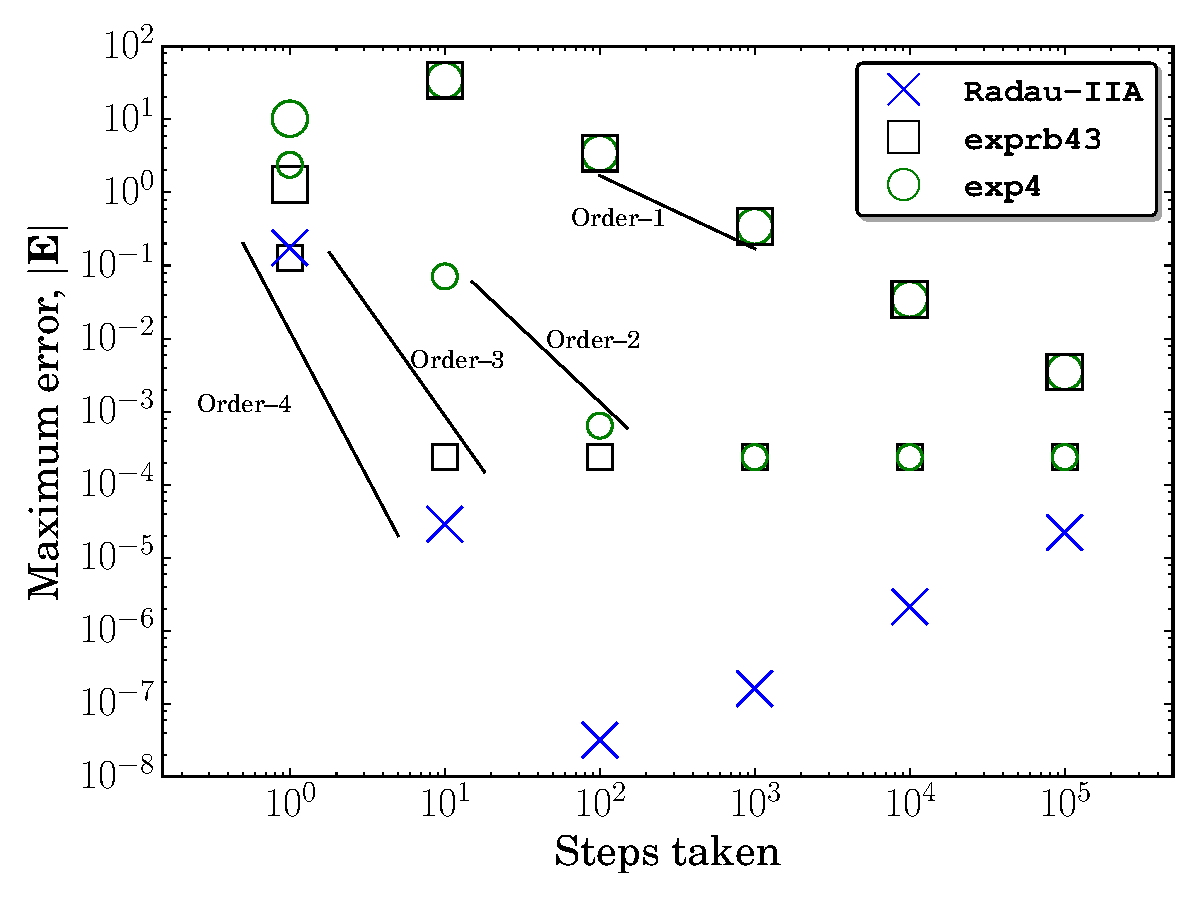
\includegraphics[width=0.7\linewidth]{c_nco_nosmem_error.pdf}
  \caption{Maximum error of the various CPU solvers as a function of the total number of integration steps taken (corresponding to decreasing time-step size).
  Larger square and circle symbols indicate the use of Krylov subspace approximations with the exponential methods, while the smaller symbols indicate the use of ``exact'' Krylov subspaces.}
  \label{F:convergence}
 \end{figure}

To investigate the correctness of the developed solvers, the first \num{10000} conditions in the \ce{H2}\slash\ce{CO} database were integrated by each solver for \SI{e-6}{\second}.
The error for condition $i$ was then determined using the weighted root-mean-square error
\begin{equation}
 E_i(t) = \left\lVert\frac{y_i(t) - \hat{y}_i(t)}{\text{atol} + \hat{y}_i(t) \times \text{rtol}}\right\rVert_2 \;,
\end{equation}
where the $y_i(t)$ is the solution obtained from the various solvers, atol\slash rtol are the absolute\slash relative tolerances, and $\hat{y}_i(t)$ is the ``true'' solution obtained via \texttt{CVODE} using a global time-step of $\delta t = \SI{e-10}{\second}$ and absolute\slash relative tolerances of \num{e-20} and \num{e-15}, respectively.
The maximum error over all conditions
\begin{equation}
 \left\lvert\textbf{E}\right\rvert = \max_{i= 1, \dots, \num{10000}}\{E_i(t)\}
\end{equation}
was then used to measure the error of each solver.
The error measurement used the same tolerances as for the performance testing ($\text{atol} = \num{e-10}$ and $\text{rtol} = \num{e-6}$, respectively).
The time-step size was then varied from \SIrange{e-6}{e-11}{\second}, using constant internal time-step sizes---corresponding to \numrange[retain-zero-exponent]{e0}{e5} time steps---to measure the convergence rates of the various solvers.

Figure~\ref{F:convergence} shows the convergence of error for the CPU solvers with decreasing time-step size, shown as increasing number of integration steps taken.
The error of the \texttt{Radau-IIA} integrator drops over four orders of magnitude when changing from a single time step of \SI{e-6}{\second} to ten time steps of \SI{e-7}{\second}, i.e., fourth order convergence.
Increasing the number of integration steps---by further reducing the time-step size---past this point does not reduce error further, due to numerical precision effects; this likely causes the apparent order reduction of the \texttt{Radau-IIA} solver, which is nominally fifth order.
The exponential solvers utilizing an approximate Krylov subspace exhibit larger levels of error in general, with $\left\lvert\textbf{E}\right\rvert \sim \mathcal{O}(1)\text{--}\mathcal{O}(10)$ for a single integration step of $\delta t = \SI{e-6}{\second}$.
As the time-step size is decreased, the convergence of the Arnoldi algorithm is affected by the internal integration time-step size (the matrix exponentials and error estimates are scaled by the internal time-step).
To study the effect of the Arnoldi algorithm on error, Fig.~\ref{F:convergence} also presents the error convergence of the exponential integrators with the Krylov approximation error reduced far below the error of the overall method.
Practically, this was accomplished by detecting when the $n$th Krylov subspace vector approaches zero, a condition known as the ``happy breakdown'' in literature~\cite{datta2010numerical}.
At this limit, the approximate exponential matrix\slash vector product approaches the exact value and thus the Krylov approximation induces negligible error.
Figure~\ref{F:convergence} shows that the exponential methods achieve only first-order convergence to the true solution with the approximate Krylov subspace, but both methods converge at higher rates with the ``exact'' Krylov subspace.
The nominal fourth-order convergence of the \texttt{exp4} algorithm is a classical nonstiff order, and thus order reduction is expected for stiff problems~\cite{ANU:7701740,Bisetti:2012jw}; the \texttt{exp4} solver reaches roughly second-order convergence with the ``exact'' Krylov subspace.
The \texttt{exprb43} solver reaches third-order convergence with the ``exact'' Krylov subspace---again, likely due to numerical precision effects, since further reduction of the time-step size does not affect error.
Furthermore, the error of Krylov subspace approximation dominates the error measurement $\lvert\textbf{E}\rvert$.
From Fig.~\ref{F:convergence} we conclude that all solvers produce reasonably accurate solutions as compared to \texttt{CVODE}.
Additionally, although not shown, the GPU solvers produce identical results.


%%%%%%%%%%%%%%%%%%%%%%%%%%%%%%%%%%%%%%%%%%%%
\section{Results and discussion}
\label{S:results}
%%%%%%%%%%%%%%%%%%%%%%%%%%%%%%%%%%%%%%%%%%%%

We studied the performance of the three integrators by testing each on the PaSR conditions described in Section~\ref{S:pasr_conditions} for two different global integration time-step sizes: $\delta t = \SI{e-6}{\s}$ and $\delta t = \SI{e-4}{\s}$.
Using a larger global time step induces additional stiffness and allows evaluation of the performance of the developed solvers on the same chemical kinetic model with varying levels of stiffness.
In reactive-flow simulations, the chemical integration time-step is typically determined by the flow time-scale and stability requirements determined by the Courant--Friedrichs--Lewy number; typical time-step values range from \SIrange{e-6}{e-1}{\s}~\cite{Yang:2013ip}.
Although the time-step size used in a given simulation depends highly on the problem and numerical methods, large-eddy simulations usually require higher time resolution than Reynolds-averaged Navier--Stokes simulations~\cite{Iaccarino:2003147}.
Hence, the time-steps chosen for study are representative of realistic values used in large-eddy~\cite{Wang20111319,Bulat20133155} and Reynolds-averaged Navier--Stokes~\cite{Ramirez2010,Galloni20091131} simulations.
Runtimes are reported as the average over five runs, where each run started from the same set of PaSR conditions.
All CPU integrators were compiled using \texttt{gcc 4.8.5} (with the compiler options ``\texttt{-O3 -funroll-loops -mtune=native}'') and executed in parallel via OpenMP on four ten-core \SI{2.2}{\giga\hertz} Intel Xeon E5-4640 v2 CPUs with \SI{20}{\mega\byte} of L3 cache memory.
OpenMP was used to parallelize on a per-condition basis; i.e., each individual OpenMP thread was responsible for integrating a single set of chemical kinetic ODEs, rather than cooperating with other OpenMP threads to solve the same.
A six-core \SI{2.67}{\giga\hertz} Intel Xeon X5650 CPU hosted the GPU integrators, which were compiled using \texttt{nvcc 7.5.17} (with compiler options ``\texttt{-arch=sm\_20 -O3 -maxrregcount 63 -{}-ftz=false -{}-prec-div=true -{}-prec-sqrt=true -{}-fmad=false}'') and run on a single NVIDIA Tesla C2075 with \SI{6}{\giga\byte} of global memory.
Reported runtimes for the GPU-based algorithms include time needed for CPU--GPU data transfer before and after each global time step; in addition, the function \texttt{cudaSetDevice()} initialized the GPU before timing to avoid any device initialization delay.
The open-source \texttt{pyJac} software~\cite{niemeyer_2016_51139,Niemeyer:2015ws,Niemeyer:2016aa} produced CPU and GPU custom source-code functions for the chemical source terms and analytical Jacobian matrix evaluation.
Finally, the L1\slash shared-memory cache was set to prefer a larger L1 cache using the \texttt{cudaDeviceSetCacheConfig()} function.

\subsection{Performance}
\label{S:perf}

For all cases in this section, the integrator runtimes are presented as the runtime per ODE solved, for two reasons.
First, saturation of the available computational resources becomes visually apparent (transition from a nearly linear decrease to a flat trend), and second, it allows certain other performance trends (e.g., the effects of thread divergence) to be easily highlighted.
The presentation of the performance data in raw form is also available in \ref{S:raw} for completeness.

\begin{figure}[htb]
  \centering
  \begin{subfigure}{0.49\textwidth}
      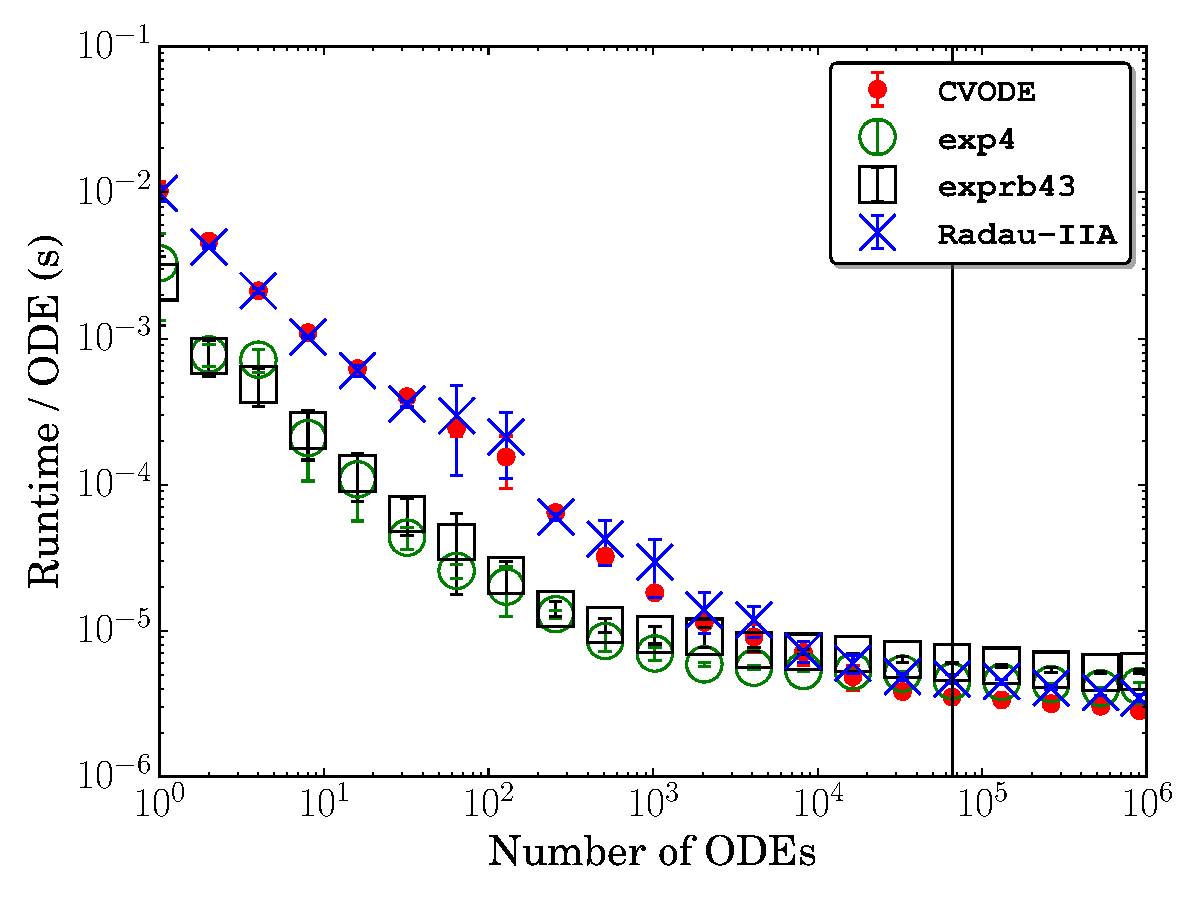
\includegraphics[width=\linewidth]{H2_1e-06_cpu.pdf}
      \caption{CPU performance for $\delta t = \SI{e-6}{\second}$}
      \label{F:h2_cpu_perf_small}
  \end{subfigure}
  %\hfill
  \begin{subfigure}{0.49\textwidth}
      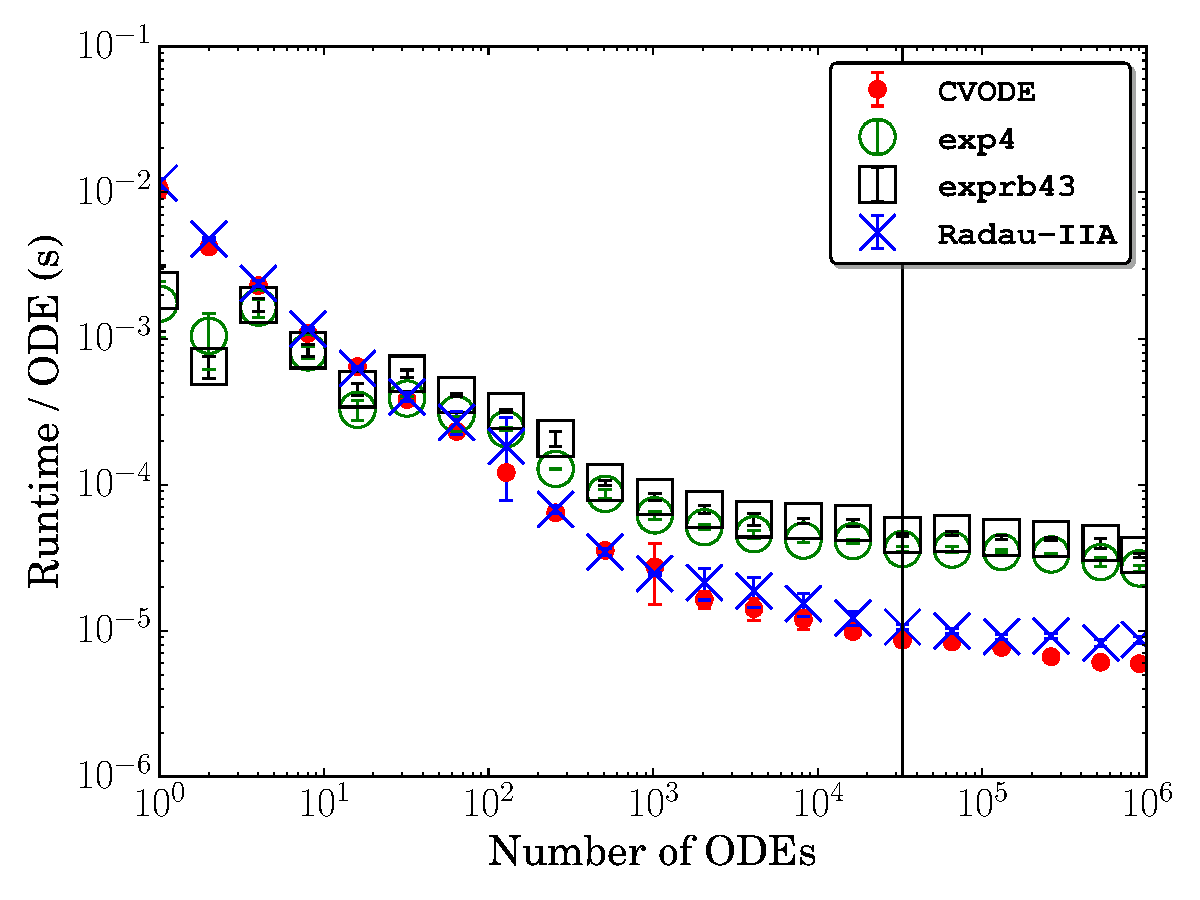
\includegraphics[width=\linewidth]{H2_1e-04_cpu.pdf}
      \caption{CPU performance for $\delta t = \SI{e-4}{\second}$}
      \label{F:h2_cpu_perf_large}
  \end{subfigure}\\
  \begin{subfigure}{0.49\textwidth}
      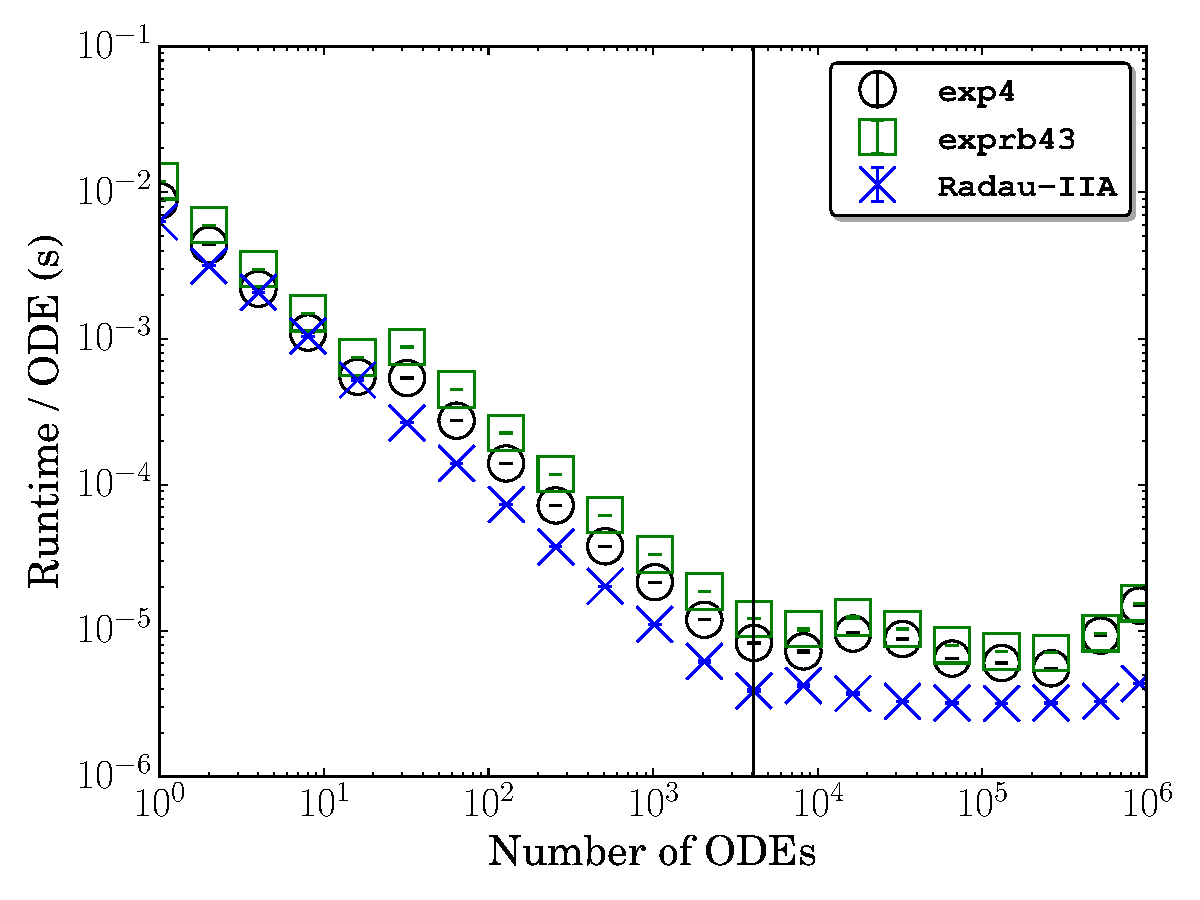
\includegraphics[width=\linewidth]{H2_1e-06_gpu.pdf}
      \caption{GPU performance results for $\delta t = \SI{e-6}{\second}$}
      \label{F:h2_gpu_perf_small}
  \end{subfigure}
  %\hfill
  \begin{subfigure}{0.49\textwidth}
      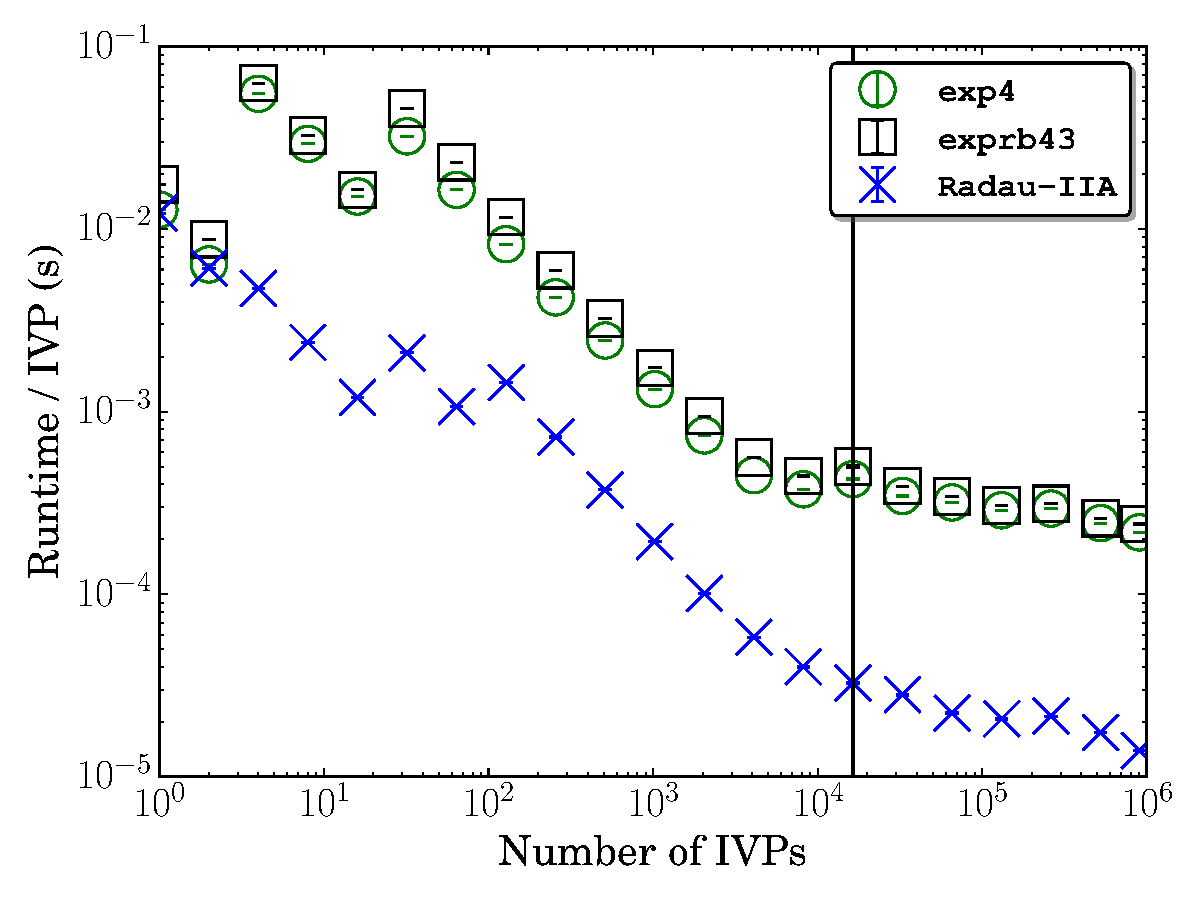
\includegraphics[width=\linewidth]{H2_1e-04_gpu.pdf}
      \caption{GPU performance results for $\delta t = \SI{e-4}{\second}$}
      \label{F:h2_gpu_perf_large}
  \end{subfigure}
  \caption{Average runtimes of the integrators on the CPU and GPU, scaled by the number of ODEs, for the \ce{H2}\slash\ce{CO} model at two different global time-step sizes.
  Estimation of where the runtime per ODE reaches a constant value (based on the results for \texttt{CVODE}\slash\texttt{Radau-IIA} for the CPU\slash GPU respectively) is marked in with a vertical line for all cases.
  Error bars indicate standard deviation.}
  \label{F:H2_perf}
\end{figure}

Figure~\ref{F:H2_perf} shows the runtimes of the CPU and GPU integrators for the \ce{H2}\slash\ce{CO} model.
In Fig.~\ref{F:h2_cpu_perf_small} the runtimes per ODE for the CPU integrators with a global time-step of $\delta t= \SI{e-6}{\second}$ decrease approximately linearly with the number of ODEs for small numbers of initial conditions (shown here on a log-log plot).
For small numbers of ODEs, the exponential integrators are faster than the implicit integration techniques due to the modest stiffness of the \ce{H2}\slash\ce{CO} model; even with many near-equilibrium states removed from the beginning of the PaSR database, the model is not particularly stiff for this small time-step size.
Larger numbers of ODEs begin to saturate the CPU resources, and the runtime per ODE levels off to a more constant value.
Eventually, relatively more stiff conditions are encountered and the performance of the implicit integration techniques catches up and then surpasses that of the exponential integrators; \texttt{CVODE} is the most efficient solver on the CPU when solving more than \num{e4} ODEs; however, \texttt{CVODE} is only $\sim$\num{1.87}$\times$ faster than the slowest solver (\texttt{exprb43}) on the whole database.
Figure~\ref{F:h2_gpu_perf_small} shows the performance of the GPU integrators for the smaller global time-step size, which exhibit similar trends as the CPU solvers: a linearly decreasing solution cost that reaches a roughly constant value beyond \numrange{e3}{e4} ODEs.
Unlike for the CPU solvers, the GPU-based \texttt{Radau-IIA} performs faster than the exponential solvers for all numbers of ODEs.
As will be seen in Section~\ref{S:divergence}, both solver classes experience minimal thread divergence due to differing internal integration time-step size in this case.
Therefore, we conclude that the relatively slower runtimes per ODE for the exponential algorithms on the GPU results from thread divergence in the Arnoldi iteration---caused by varying Krylov subspace sizes between threads.

Figures~\ref{F:h2_cpu_perf_large} and \ref{F:h2_gpu_perf_large} show the performance of the integration algorithms on both platforms for the \ce{H2}\slash\ce{CO} model with the larger global time-step size ($\delta t=\SI{e-4}{\second}$).
The performances of the CPU integration algorithms show similar trends to those of the smaller time-step size case: decreasing cost per ODE before reaching a more constant performance for higher numbers of ODEs.
The larger time-step size induces additional stiffness, and the implicit solvers are more efficient for most numbers of ODEs; \texttt{CVODE} is again the most efficient CPU solver.
Fig.~\ref{F:h2_gpu_perf_large} shows the performance of the GPU solvers for the larger global time-step size.
The exponential solvers exhibit significant spikes in computational cost when changing from 2--4 and 16--32 ODEs, with the latter mimicked somewhat by the implicit \texttt{Radau-IIA} solver.
A jump in solution cost between 2--4 ODEs is also present for the CPU exponential integrators, indicating chemical stiffness as the primary cause.
On the other hand, between 16--32 ODEs the CPU exponential solvers exhibit only a very minor performance decrease, while the GPU-based \texttt{Radau-IIA} also shows a decrease in performance at the same point---a trend completely absent in the CPU \texttt{Radau-IIA} version.
These factors indicate that thread divergence also plays a key role in the performance trend here, and will be investigated further in Section~\ref{S:divergence}.
As in case of the smaller global time-step size, the \texttt{Radua-IIA} solver is the most efficient GPU algorithm in all cases.

\begin{figure}[htb]
  \centering
  \begin{subfigure}{0.49\textwidth}
      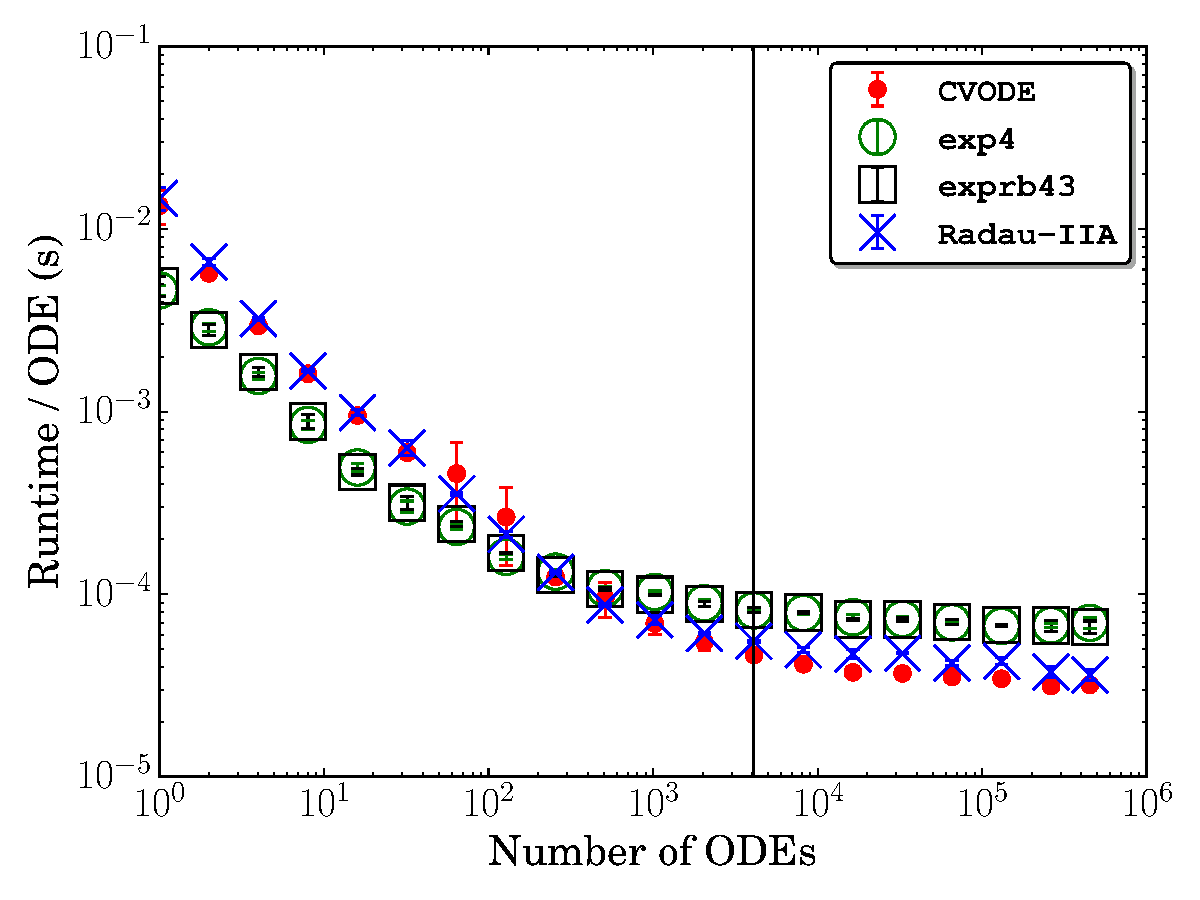
\includegraphics[width=\linewidth]{CH4_1e-06_cpu.pdf}
      \caption{CPU performance for $\delta t = \SI{e-6}{\second}$}
      \label{F:ch4_cpu_perf_small}
  \end{subfigure}
  %\hfill
  \begin{subfigure}{0.49\textwidth}
      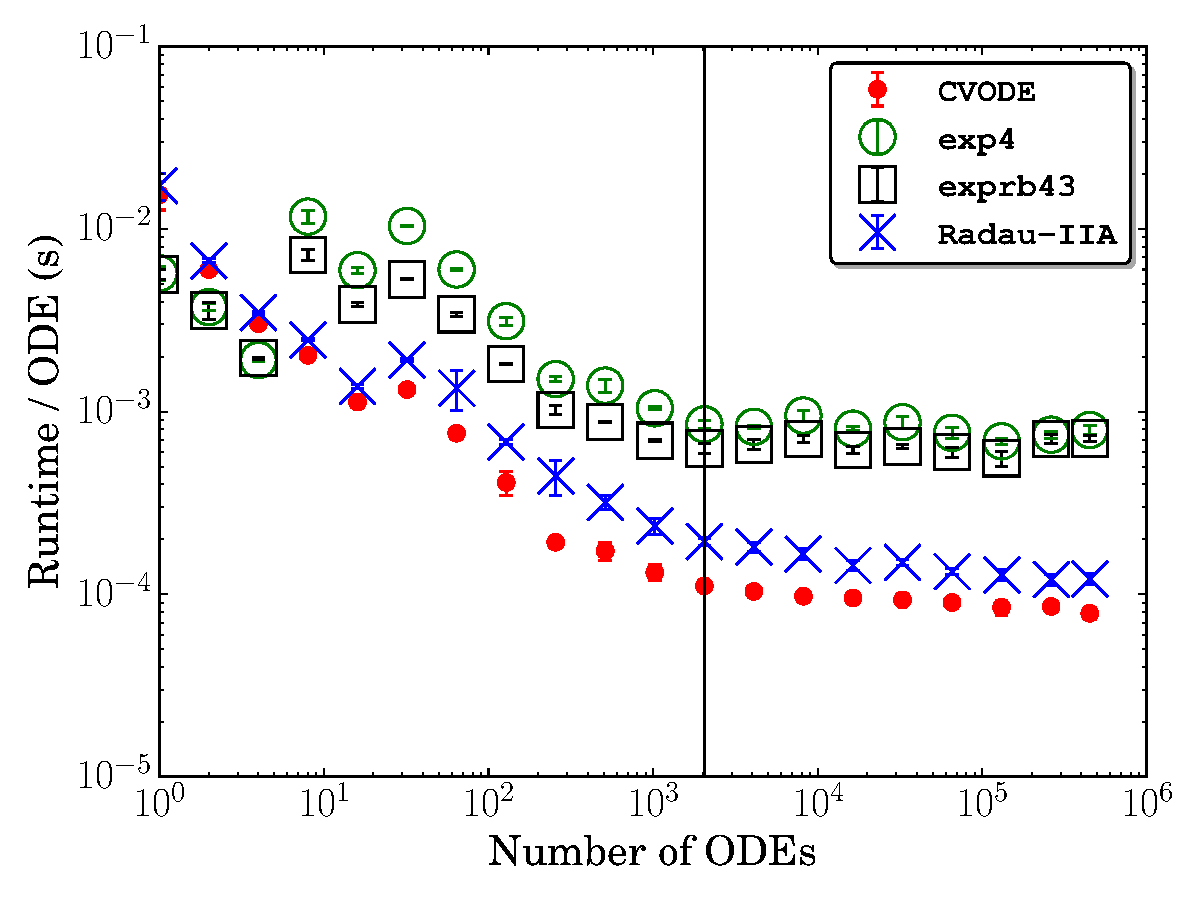
\includegraphics[width=\linewidth]{CH4_1e-04_cpu.pdf}
      \caption{CPU performance for $\delta t = \SI{e-4}{\second}$}
      \label{F:ch4_cpu_perf_large}
  \end{subfigure}\\
  \begin{subfigure}{0.49\textwidth}
      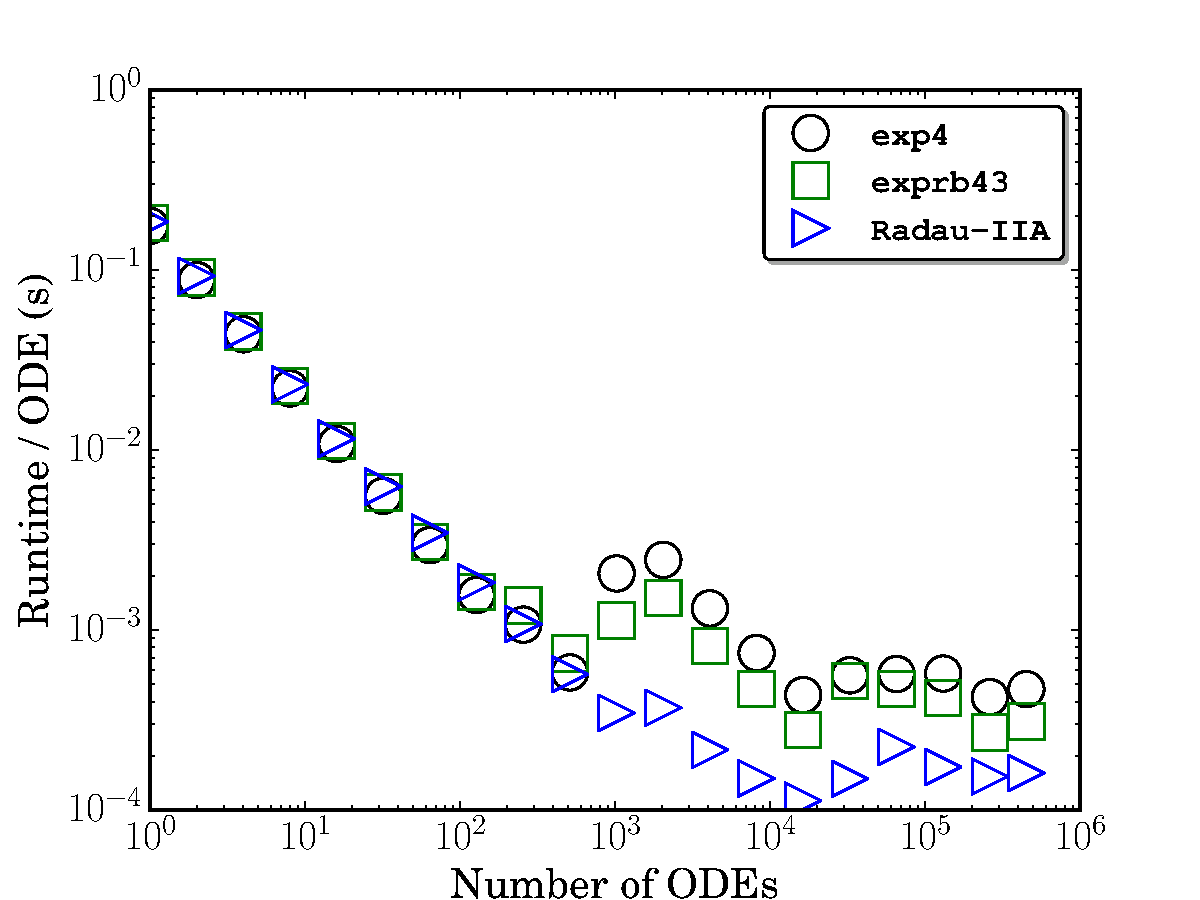
\includegraphics[width=\linewidth]{CH4_1e-06_gpu.pdf}
      \caption{GPU performance results for $\delta t = \SI{e-6}{\second}$}
      \label{F:ch4_gpu_perf_small}
  \end{subfigure}
  %\hfill
  \begin{subfigure}{0.49\textwidth}
      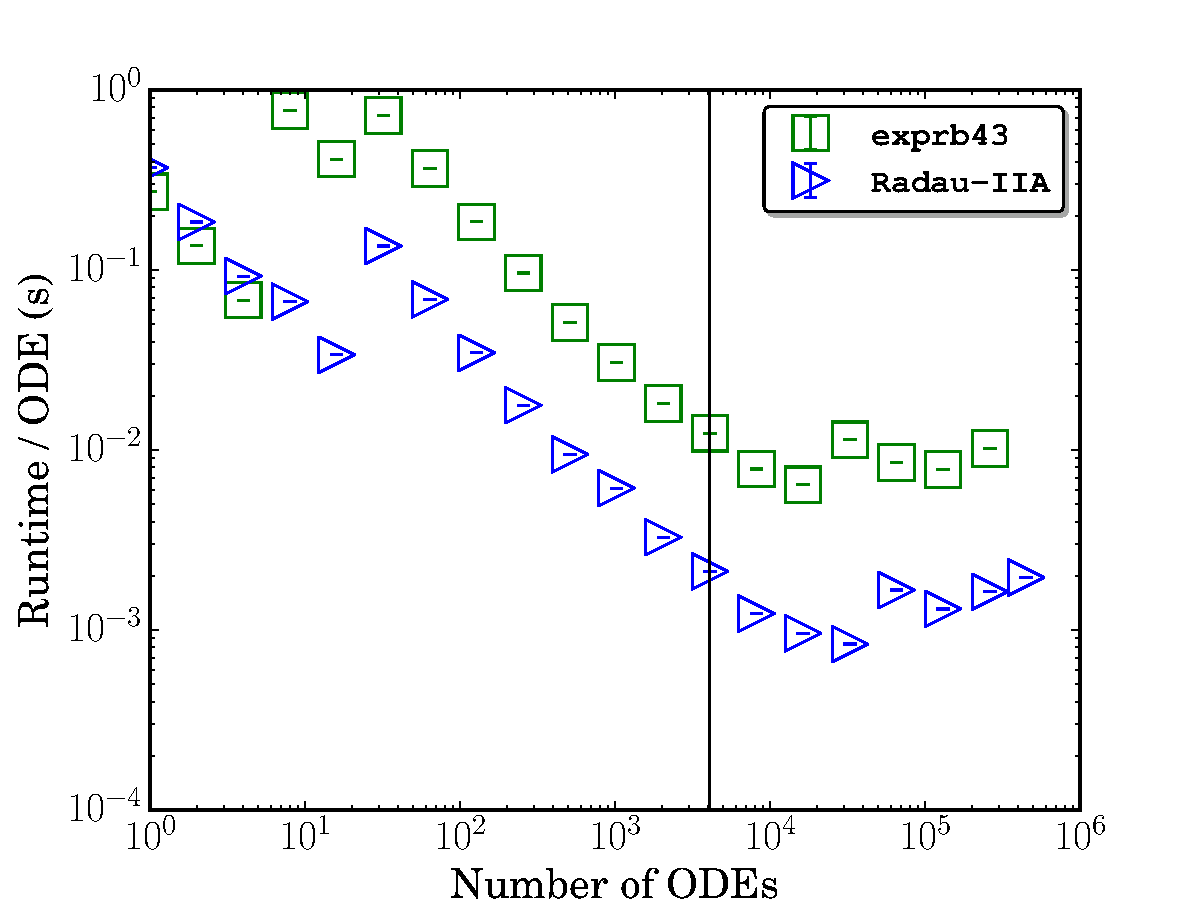
\includegraphics[width=\linewidth]{CH4_1e-04_gpu.pdf}
      \caption{GPU performance results for $\delta t = \SI{e-4}{\second}$}
      \label{F:ch4_gpu_perf_large}
  \end{subfigure}
  \caption{Average runtimes of the integrators, scaled by number of ODEs, on the CPU and GPU for the GRI-Mech 3.0 model at two different global time-step sizes.
  Estimation of where the runtime per ODE reaches a constant value (based on the results for \texttt{CVODE}\slash\texttt{Radau-IIA} for the CPU\slash GPU respectively) is marked in with a vertical line for all cases.
  Error bars indicate standard deviation.}
  \label{F:CH4_perf}
\end{figure}

Figure~\ref{F:CH4_perf} shows the runtime of the integrators for the GRI-Mech 3.0 model.
Similar to the \ce{H2}\slash\ce{CO} case for the smaller global time-step size, the CPU exponential integrators are more efficient (Fig.~\ref{F:ch4_cpu_perf_small}) for the near-equilibrium conditions at the beginning of the database.
For larger numbers of conditions, the implicit integrators are more efficient, and \texttt{CVODE} again performs the fastest.
Compared to the \ce{H2}\slash\ce{CO} model (Fig.~\ref{F:h2_cpu_perf_small}), the \texttt{CVODE} performs better than the exponential algorithms for the GRI-Mech 3.0 model with the small global time-step size (Fig.~\ref{F:ch4_cpu_perf_small}), reaching a speedup of \SI{2.18}{$\times$} over \texttt{exp4} on the whole database; this results from the higher stiffness present in the model.
This performance gap between the CPU implicit\slash exponential integrators increases for the larger global time-step size (Fig.~\ref{F:ch4_cpu_perf_large}); \texttt{CVODE} is \SI{10.1}{$\times$} faster than \texttt{exp4} on the whole database.
Comparing the performance of the CPU implicit solvers between the two kinetic models shows roughly an order-of-magnitude performance decrease for both global time-step sizes.
This phenomena, due largely to the increase in model size, is also seen for the \texttt{Radau-IIA} GPU solver for the smaller global time-step size; the performance of which decreases by just over an order of magnitude.
However, for the larger global time-step size, the GPU-based \texttt{Radau-IIA} solver performs roughly two orders-of-magnitude slower compared with the \ce{H2}\slash\ce{CO} case.
As will be examined in Section~\ref{S:divergence}, this dramatic decrease likely results from increased thread divergence in the \texttt{Radau-IIA} solver, as well as the increased memory traffic inherent in the larger model.

Unlike for the \ce{H2}\slash\ce{CO} model, the \texttt{exprb43} solver outperforms \texttt{exp4} with the GRI-Mech 3.0 model in almost all cases for the larger time-step size for both the CPU and GPU.
Although the \texttt{exprb43} and \texttt{exp4} algorithms each require three exponential matrix function approximations per step, a single internal time step of \texttt{exprb43} is more expensive due to the extra chemical source term evaluations, matrix multiplications, and higher-order exponential matrix function requirement.
As such, the relatively simpler CPU \texttt{exp4} integrator outperforms the CPU \texttt{exprb43} integrator for the \ce{H2}\slash\ce{CO} model where there is relatively less chemical stiffness.
However, as previously discussed the \texttt{exp4} algorithm may experience order reduction for stiff problems, and the \texttt{exprb43} algorithm typically outperforms \texttt{exp4} on both the CPU and GPU in the larger global time-step GRI-Mech 3.0 case as a result.


% The GPU \texttt{Radau-IIA} integrator outperformed \texttt{CVODE} for the smaller time-step size; at best, it ran \SI{31.5}{\percent} faster than \texttt{CVODE} (\num{131072} ODEs), and at worst was \SI{10}{\percent} faster (\num{16384} ODEs).
% The larger time-step size again negatively impacted the performance of the GPU-based \texttt{Radau-IIA} integrator, dropping the performance to \num{8.63}$\times$ slower than \texttt{CVODE} at best (\num{32768} ODEs), and \num{20.5}$\times$ slower in the worst case (\num{450900} ODEs).
% For the smaller time-step size the CPU \texttt{Radau-IIA} integrator was \SI{13}{\percent} faster than \texttt{CVODE} at best (\num{131072} ODEs) and \SI{10}{\percent} faster at worst (\num{450900} ODEs).
% The larger time-step size---the stiffest case---was the only case where \texttt{CVODE} significantly outperformed CPU \texttt{Radau-IIA}, which was \num{2.66}$\times$ slower at best (\num{65536} ODEs) and \num{4.11}$\times$ slower at worst (\num{450900} ODEs).
% This difference may be due to the adaptive-order nature of the \texttt{CVODE} algorithm, or potentially due to its maturity and years of optimization.
% However, this effect is fairly minor and should not cause the order-of-magnitude decrease in relative performance between the GPU-based \texttt{Radau-IIA} integrator and \texttt{CVODE} observed when switching to the larger time step.

\subsection{CPU\slash GPU performance comparison}

Comparing the performance of CPU- and GPU-based integrators in a meaningful way is challenging.
First, the vastly different nature of the processing cores in each platform eliminates the possibility of comparing performance normalized by core count.
In addition, the floating-point operation count is not readily available for chemical kinetic integration---unlike many GPU-accelerated applications where the number of operations required to solve the problem is known, e.g., as in linear-algebra operations or fast Fourier transforms---which precludes comparing performance on the basis of floating-point operations per second (FLOPS).
Although the runtimes of the GPU integration algorithms can be directly compared with that of the CPU-based solvers (and often are), these figures do not provide much useful information.
For instance, if a GPU algorithm performs $\SI{10}{\times}$ faster than its equivalent on two six-core CPUs, how does this compare to two eight-core CPUs, etc.?

For researchers in numerical combustion, two issues stand out as particularly important for performance evaluation: runtime and cost.
As established in Section~\ref{sec:Intro}, large-scale reactive-flow simulations with realistic chemical kinetic models are extremely computationally expensive, and remain outside of the capabilities of most in the field.
With this in mind, we ask, for a given simulation, what is the effect on the overall runtime of adding more CPU cores compared with adding GPU accelerators?
In addition, if a budget is allocated to expand available computational resources, how might these funds be best allocated?
To answer these questions, we attempt to derive a rough estimate of the number of CPU cores required for equivalent performance on the GPU.

A nominal performance metric for both the CPU- and GPU-based integration algorithms must first be obtained.
As the most efficient solvers in all cases with large numbers of ODEs are \texttt{CVODE} for the CPU and \texttt{Radau-IIA} for the GPU, these algorithms will be considered the performance benchmarks.
Furthermore, most large-scale simulations consist of millions of cells (or more), and therefore we only consider the performance limit of each algorithm (i.e., the cost per ODE of each algorithm in the region where this cost reaches an approximately constant value).
To this end, Figs.~\ref{F:H2_perf} and \ref{F:CH4_perf} show vertical lines where the relative change in runtime per ODE between successive data-points is first smaller than \SI{15}{\percent} (based on \texttt{CVODE}\slash\texttt{Radau-IIA} for the CPU\slash GPU accordingly).
The cost per ODE above and including these thresholds was averaged and forms our nominal performance measure.
The CPU performance measure must also be normalized by the total number of cores used: \num{40}.
Table~\ref{T:cpu_equiv} presents the ratios of these performance measures, which give rough estimates for the number of CPU cores required to equal the GPU performance for the cases studied.
The GPU is roughly equivalent to \num{10} or more CPU cores for all cases except GRI-Mech 3.0 with the larger time-step size, and equivalent to at most $\sim$\num{35} cores for the \ce{H2}\slash\ce{CO} case with the smaller time-step size.

\begin{table}[htb]
\centering
\begin{tabular}{@{}l S[table-format=2.1] S[table-format=2.1] @{}}
\toprule
\multirow{2}{*}{Global time-step size} & \multicolumn{2}{c}{\# equivalent CPU cores} \\ \cmidrule{2-3}
 & \ce{H2}\slash\ce{CO} & \ce{GRI-Mech 3.0} \\
\midrule
\SI{e-6}{\second} & 35.4 & 10.4 \\
\SI{e-4}{\second} & 14.0 & 2.6 \\
\bottomrule
\end{tabular}
\caption{The number of CPU cores (roughly) required for equivalent performance to a single GPU for the combinations of chemical kinetic models and global time-step sizes studied.}
\label{T:cpu_equiv}
\end{table}

Finally, at the time of writing, the ten-core Intel Xeon E5-4640 v2 CPU used in this study was listed for a recommended customer price of \SI{2725}[\$]{}~\cite{intel_price}, while a new Tesla C2075 GPU is available for $\sim$\SI{1400}[\$]{}~\cite{gpu_price}.
These prices are only rough estimates of the actual cost of these devices, since the actual price for the Intel CPU may be significantly less in a configured server node, while the Tesla C2075 is no longer sold directly by NVIDIA---thus the prices are variable.
Furthermore, the performance decrease using an older, cheaper CPU (e.g., the Intel Xeon X5650 used as host processor for the GPU simulations in this work) may not be that large.
However, combined with the equivalent core counts in Table~\ref{T:cpu_equiv}, this information suggests that the Tesla C2075 is a reasonable investment to supplement computing power for chemical-kinetic integration in large-eddy simulations.
For the global time-step size of \SI{e-4}{\second}, corresponding to Reynolds-averaged simulations, the benefit is less clear for the stiffer GRI-Mech 3.0 model.
More work is required in thread divergence avoidance and memory traffic reduction to improve the GPU performance in this case.


\subsection{Effect of thread divergence}
\label{S:divergence}

Thread divergence and memory traffic are two performance concerns particularly important for chemical kinetic integration on SIMD platforms.
Slowdown due to memory traffic for a GPU integration algorithm implemented on a per-thread basis primarily results from the small amount of on-chip memory available.
Reformulating the chemical kinetic equations to generate sparse Jacobian matrices~\cite{Schwer2002270} would likely benefit GPU-based integration algorithms due to the reduced memory requirements; this is a planned improvement to the \texttt{pyJac} software~\cite{Niemeyer:2016aa,niemeyer_2016_51139}.
The performance penalty due to thread divergence depends both on the cost of the divergent branches as well as the proportion of the warp that executes each branch.
For example, if only one thread in a warp executes an expensive branch (e.g., a Jacobian update) the rest of the warp remains idle during that time, and the SM may become severely underutilized.

To investigate the effects of thread divergence further, we adopted a modified version of the quantification of thread divergence of Niemeyer and Sung~\cite{Niemeyer:2014aa}:
\begin{equation}
	D = 1 - \frac{\sum_{i=1}^{32}{d_i}}{32 \times \max\limits_{i = 1, \dots, 32} d_i} \;,
	\label{eqn:divergence}
\end{equation}
where $d_i$ is the number of internal integrator time steps taken to reach the global time step by thread $i$ in a warp (which consists of 32 threads).
$D$ represents the similarity of internal time step counts across threads in a warp---a significant source of thread divergence.
If all threads in a warp use identical internal integration time steps and thus the warp experiences no thread divergence from this source, then $D = 0$; however, if a warp experiences an unbalanced number of internal integration time steps, then $D \to 1$.
Differing internal time-step sizes is not the only source of thread divergence for the GPU integration algorithms.
For instance, threads in a warp may use different Krylov subspace sizes for the exponential integrators or different numbers of Newton iterations for the \texttt{Radau-IIA} solver.
Indeed, Section~\ref{S:perf} notes that we suspect thread divergence from differing Krylov subspace sizes as the reason the exponential solvers are less efficient for small numbers of ODEs for the \ce{H2}\slash\ce{CO} model with the small global time-step size.
However, these operations clearly cost less than an entire internal integration step (in which they are embedded) and thus we look only at the thread divergence of internal integration time steps.
Investigation of thread divergence for such operations within a internal integration step is an important consideration and will be explored in our future work.

\begin{figure}[htbp]
  \centering
  \begin{subfigure}{0.49\textwidth}
      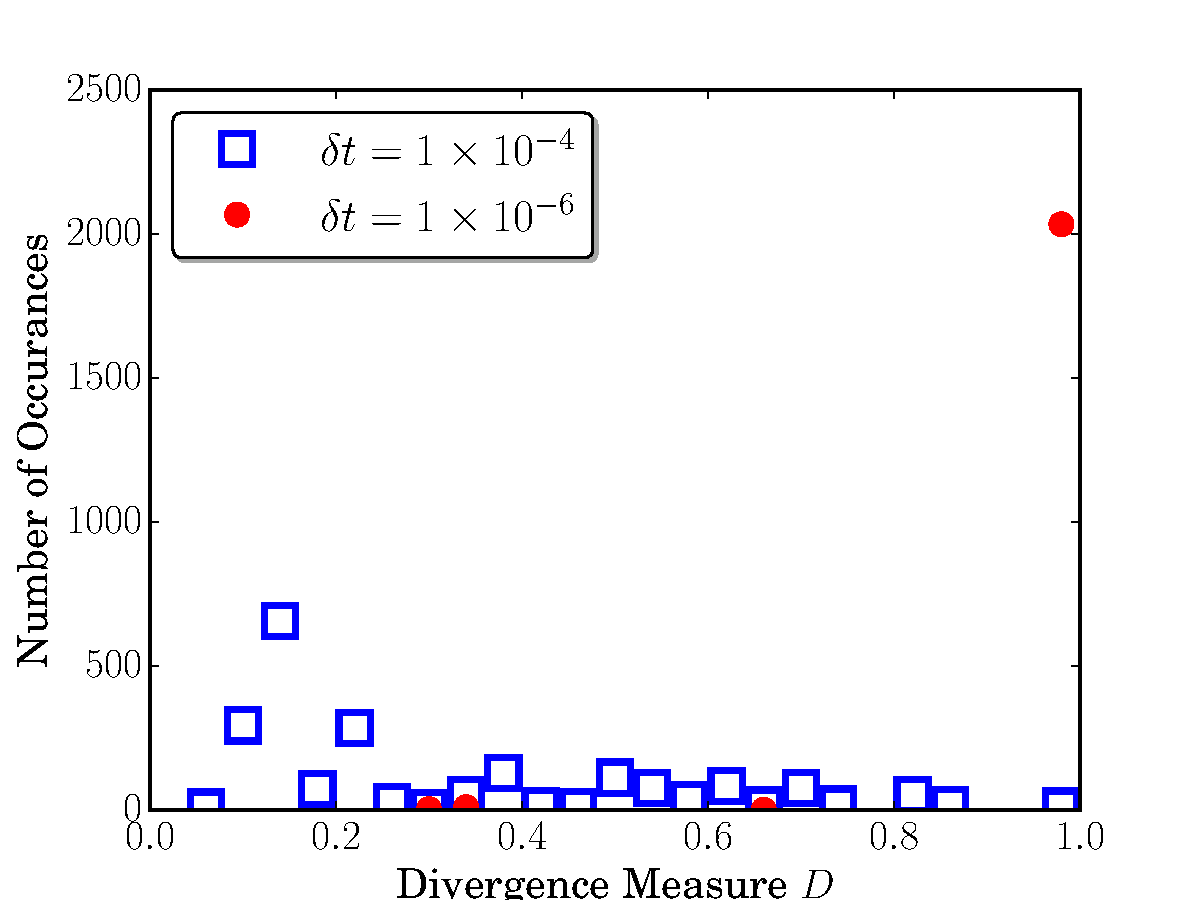
\includegraphics[width=\linewidth]{H2_radau2a_div.pdf}
      \caption{\texttt{Radau-IIA} solver for \ce{H2}\slash\ce{CO} model}
      \label{F:Rad_div_h2}
  \end{subfigure}
  %\hfill
  \begin{subfigure}{0.49\textwidth}
      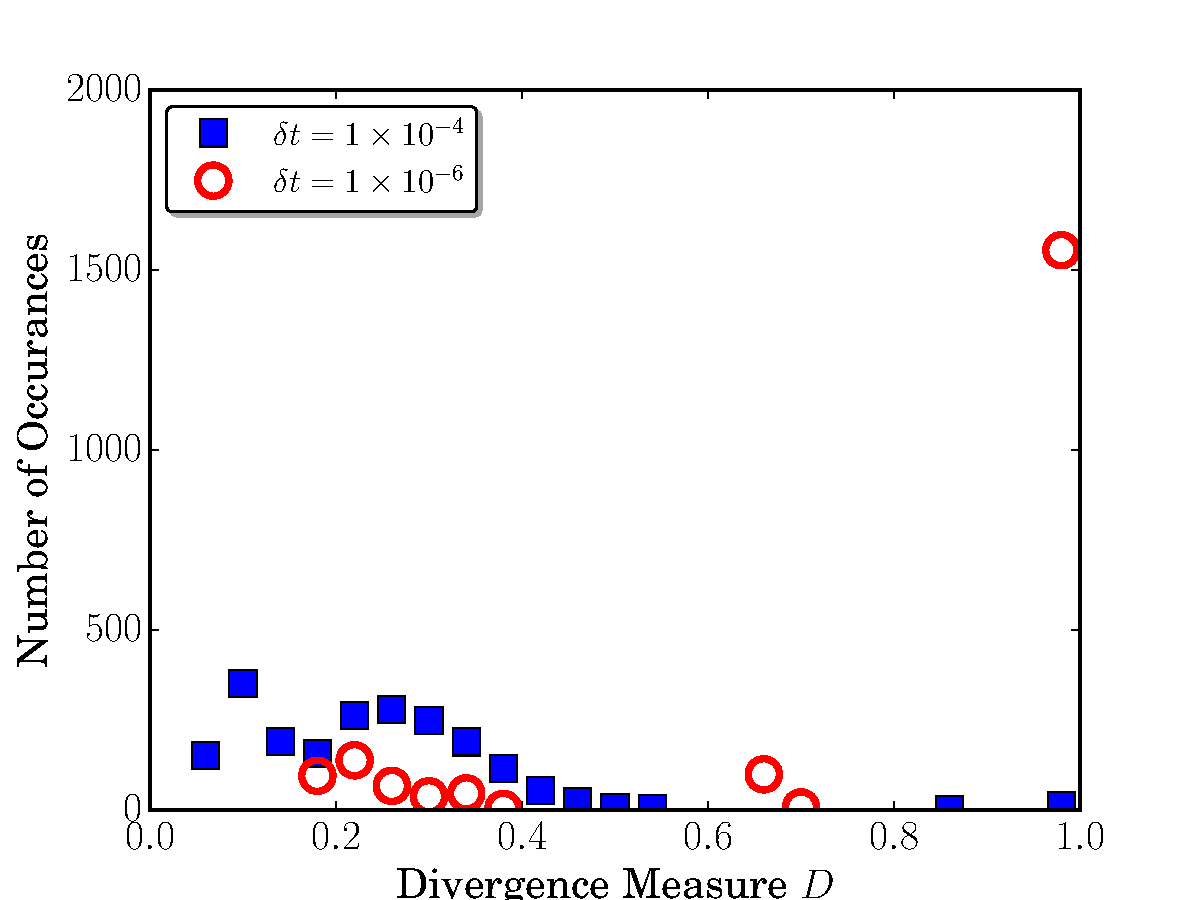
\includegraphics[width=\linewidth]{CH4_radau2a_div.pdf}
      \caption{\texttt{Radau-IIA} solver for GRI-Mech 3.0 model}
      \label{F:Rad_div_gri}
  \end{subfigure}
  \\
  \begin{subfigure}{0.49\textwidth}
      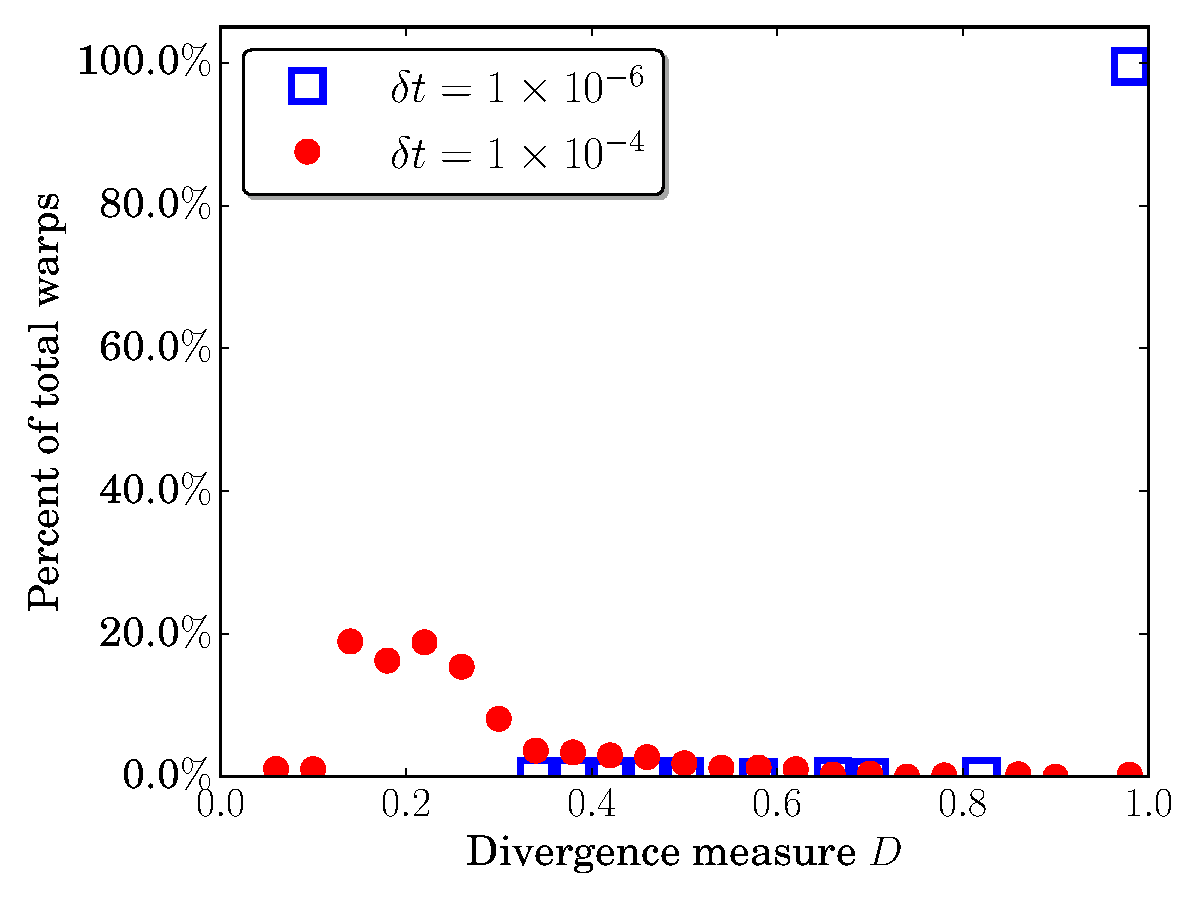
\includegraphics[width=\linewidth]{H2_exprb43_div.pdf}
      \caption{\texttt{exprb43} solver for \ce{H2}\slash\ce{CO} model}
      \label{F:exprb43_div_h2}
  \end{subfigure}
  %\hfill
  \begin{subfigure}{0.49\textwidth}
      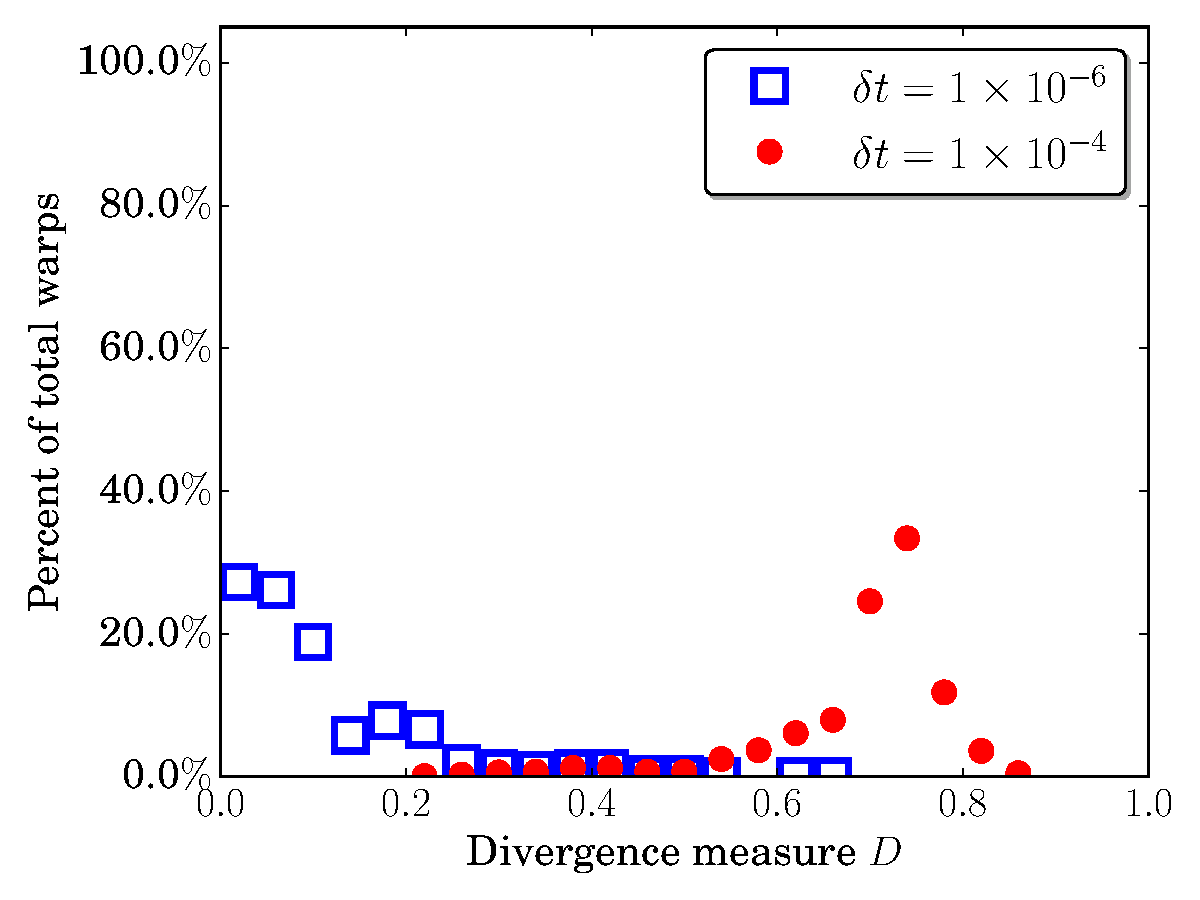
\includegraphics[width=\linewidth]{CH4_exprb43_div.pdf}
      \caption{\texttt{exprb43} solver GRI-Mech 3.0 model}
      \label{F:exprb43_div_ch4}
  \end{subfigure}
  \\
  \begin{subfigure}{0.49\textwidth}
      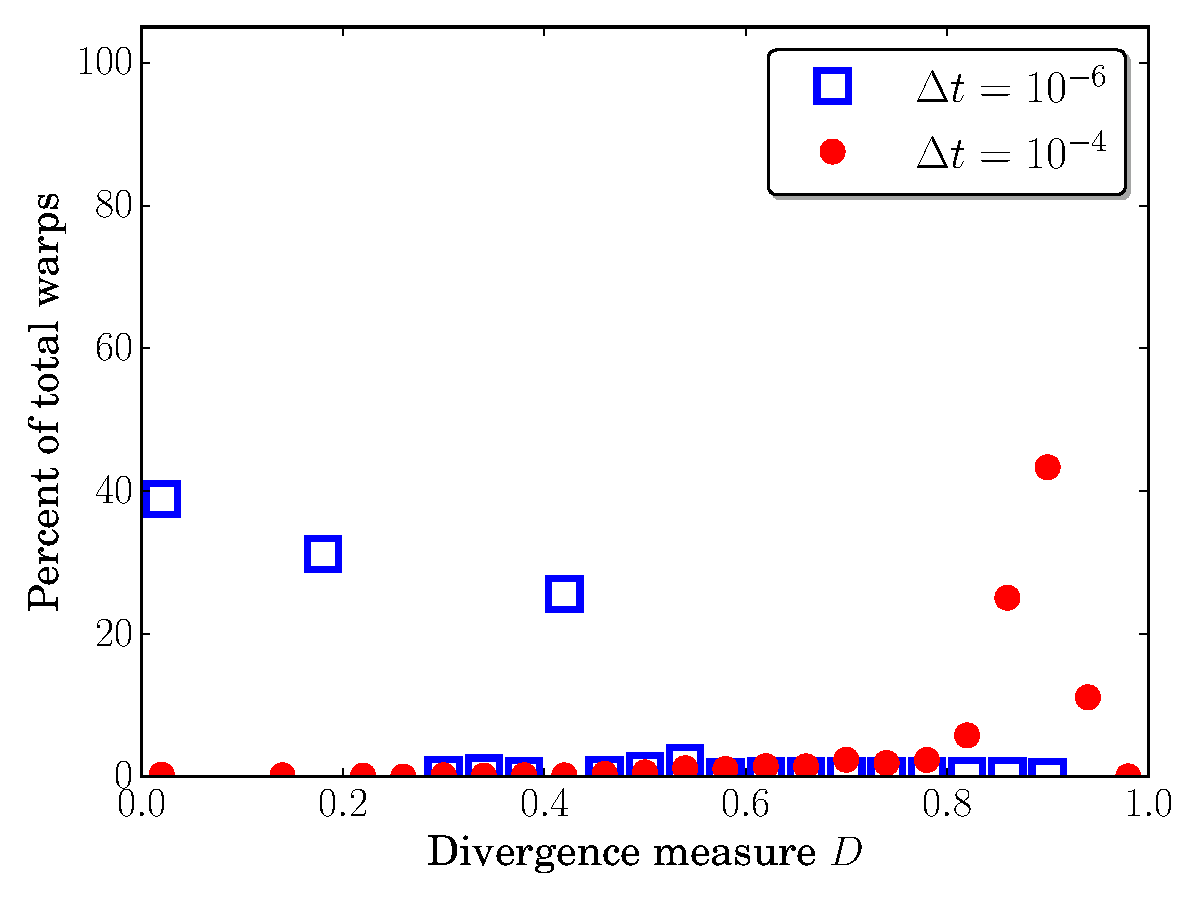
\includegraphics[width=\linewidth]{H2_exp4_div.pdf}
      \caption{\texttt{exp4} solver \ce{H2}\slash\ce{CO} model}
      \label{F:exp4_div_h2}
  \end{subfigure}
  %\hfill
  \begin{subfigure}{0.49\textwidth}
      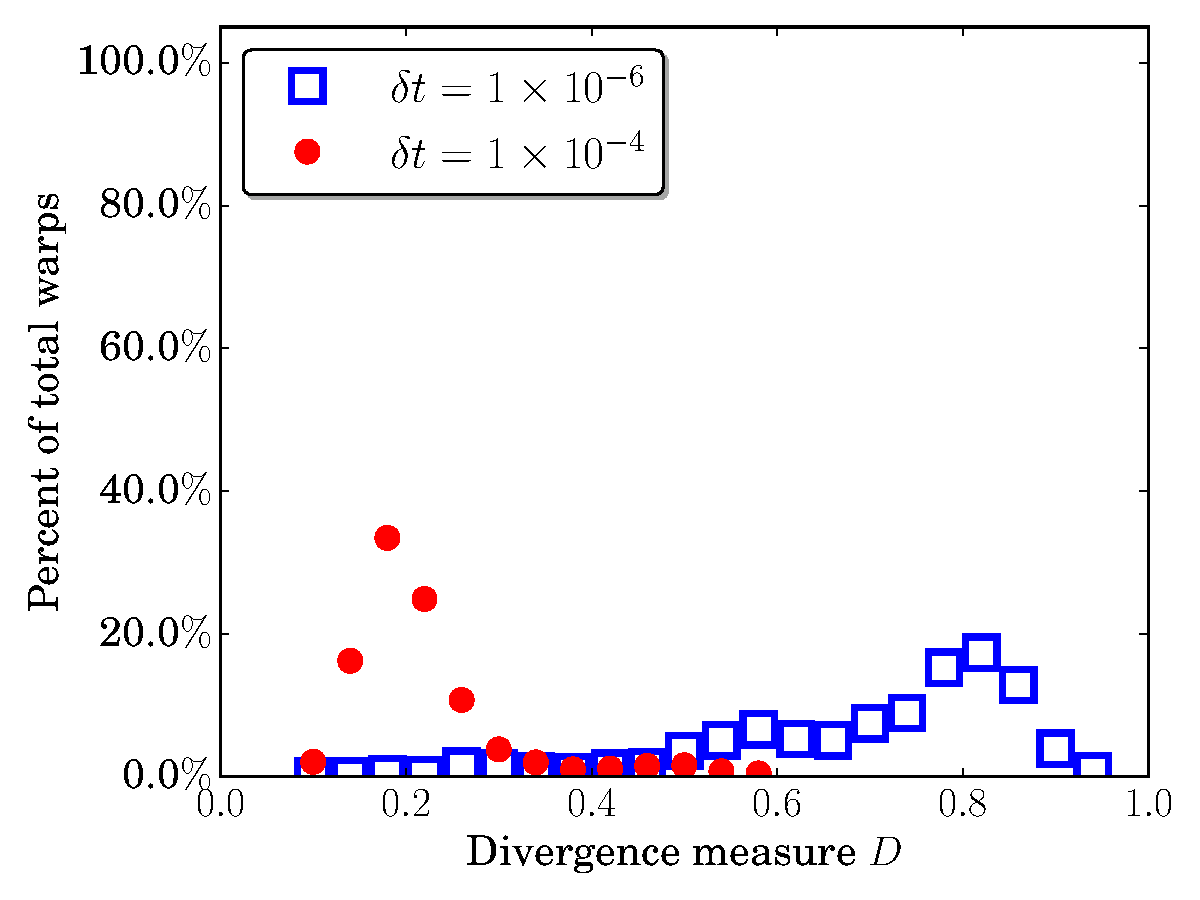
\includegraphics[width=\linewidth]{CH4_exp4_div.pdf}
      \caption{\texttt{exp4} solver GRI-Mech 3.0 model}
      \label{F:exp4_div_ch4}
  \end{subfigure}
  \caption{Thread divergence estimate for the various solvers for both models and time-step sizes.}
  \label{F:divergence}
\end{figure}

Figures~\ref{F:Rad_div_h2} and~\ref{F:Rad_div_gri} show the distribution of the divergence measure $D$ for the \texttt{Radau-IIA} solver with both global time-step sizes and kinetic models when run on \num{262144} ODEs, spread across \num{8192} warps.
For both kinetic models with the small global time-step size, nearly \SI{100}{\percent} of the warps had a divergence measure near zero.
Increasing the global time-step size causes the number of warps with high levels of thread divergence (e.g. $D > 0.5$) to increase for both models.
For the \ce{H2}\slash\ce{CO} model, over \SI{40}{\percent} of warps were between $D=0.55$ and $D=0.65$, while over \SI{75}{\percent} of warps were between $D=0.6$ and $D=0.8$ for the GRI-Mech 3.0 model.
Correspondingly, the approximate equivalent CPU core-count (Table~\ref{T:cpu_equiv}) dropped by \SI{2.5}{$\times$} for the \ce{H2}\slash\ce{CO} model at the larger global time-step sizes.
Furthermore, the GRI-Mech 3.0 model experiences higher levels of thread divergence for the larger global time-step size, and subsequently experienced a higher drop in performance of \SI{4}{$\times$}.
This observation motivates future work aimed at developing strategies to reduce thread divergence.
Potential solutions include adopting an ODE per-block approach~\cite{Stone:2013aa}, reordering ODEs to increase similarity of stiffness inside a warp, or synchronizing internal time-step sizes between threads in a warp.
However, Figs.~\ref{F:Rad_div_h2} and \ref{F:Rad_div_gri} do not explain the drop in equivalent core count between the \ce{H2}\slash\ce{CO} model and the GRI-Mech 3.0 model for the smaller global time-step size.
This likely results from a combination of thread divergence inside the internal integration step and the increased memory traffic of the larger model; this further motivates development of a sparse version of the \texttt{pyJac} software.

Figures~\ref{F:exprb43_div_h2} and \ref{F:exprb43_div_ch4} show the divergence levels of the \texttt{exprb43} GPU solver.
Similar to the \texttt{Radau-IIA} solver, nearly \SI{100}{\percent} of warps for the \texttt{exprb43} solver have no thread divergence due to differing internal integration step sizes for the \ce{H2}\slash\ce{CO} model.
The \texttt{exprb43} thread divergence levels increase somewhat for the GRI-Mech 3.0 model with the smaller time-step size; \SI{27}{\percent} of warps still had a divergence measure of $D=0$, but over \SI{63}{\percent} of the warps had divergence measures between \numrange{0.05}{0.2}.
With the larger time-step size, the \texttt{exprb43} solver experiences significantly more thread divergence for both models.
The divergence measure distribution is fairly similar to that of the \texttt{Radau-IIA} solver for the GRI-Mech 3.0 model, but most warps experience a divergence measure of $D \sim 0.8$ for the \ce{H2}\slash\ce{CO} model (versus $D \sim 0.6$ for the \texttt{Radau-IIA} solver).
The explicit solvers deal with stiffness less efficiently, and end up using a greater range of internal time-step sizes between conditions of varying stiffness.
This results in an increase in thread divergence levels due to differing internal time-step sizes.

The relatively worse stiffness handling of the \texttt{exp4} method is also apparent in Figs~\ref{F:exp4_div_h2} and \ref{F:exp4_div_ch4}; in most cases, significantly more thread divergence is seen for \texttt{exp4} than for either of the other solvers.
The \texttt{exp4} algorithm is the only solver to show significant thread divergence even for the \ce{H2}\slash\ce{CO} model for the smaller global time-step size.
Further, the \texttt{exp4} algorithm experiences more thread divergence than the \texttt{exprb43} for both models at the larger global time-step size.

\subsection{Effect of using a finite-difference-based chemical kinetic Jacobian}

While it is well established that using an analytical Jacobian matrix can significantly accelerate chemical kinetic integration on the CPU~(e.g., \cite{Lu:2009gh,stone2014comparison,Schwer2002270}), relatively little study has been directed at use of a GPU-based analytical Jacobian.
Dijkmans et al.~\cite{Dijkmans:2014bb} used a GPU-based analytical Jacobian code to accelerate various CPU-based chemical kinetic integration schemes, and our own previous works~\cite{Niemeyer:2016aa,Niemeyer:2015ws} have detailed the performance of \texttt{pyJac}.
However, to our knowledge no work using an analytical Jacobian for GPU-based chemical kinetic integration has been published.
In this section, we explore the relative performance benefits of the analytical Jacobian compared to a first-order finite-difference Jacobian on both the CPU and GPU.
The exponential methods require an exact Jacobian matrix (rather than an approximation as given by finite-difference methods), so their performance was not considered in this section.

Figure~\ref{F:AJ_comp} shows the speedup achieved on both the CPU and GPU for the \texttt{Radau-IIA} algorithm for various cases; the GRI-Mech 3.0 results for the larger global time-step have been omitted due to long run times.
For the \ce{H2}\slash\ce{CO} model (Figs.~\ref{F:AJ_h2_small} and~\ref{F:AJ_h2_large}), using the analytical Jacobian offers minimal performance benefit for the CPU-based integrators, reaching a maximum speedup of \SI{1.49}{$\times$} and \SI{1.39}{$\times$} for the small and large global time-step sizes, respectively.
This results from both the relatively small size of the model (and resulting modest chemical source-term evaluation costs), as well as the lower chemical stiffness that requires only a few Jacobian evaluations for the \texttt{Radau-IIA} solver.
In some cases the finite-difference Jacobian solver may be faster than the analytical Jacobian solver; although it is difficult to explain the exact cause of this phenomena, differences in the finite-difference Jacobian likely caused the integrator to follow a slightly different instruction path (e.g., with fewer Jacobian updates\slash chemical source term evaluations) changing the integration cost.
However, for large numbers of conditions, the analytical-Jacobian-based CPU solver indeed performs faster than the finite-difference counterpart.
In contrast, the analytical-Jacobian-based GPU solver performs significantly faster than the finite-difference GPU solver in all cases for the \ce{H2}\slash\ce{CO} model, reaching a maximum speedup of \SI{12.16}{$\times$} for the smaller global time-step size.
As discussed in Section~\ref{S:divergence}, significantly higher levels of thread divergence are expected for the larger global time-step size.
Correspondingly, the maximum speedup of the GPU solver increases to \SI{240.96}{$\times$} for the larger global time-step size.
Figure~\ref{F:AJ_ch4_small} shows that the speedup of the CPU and GPU solvers reach \SI{2.61}{$\times$} and \SI{7.11}{$\times$}, respectively, for the larger GRI-Mech 3.0 model at the smaller global time-step size.
It is clear that for a per-thread-based GPU integrator, using an analytical Jacobian is essential for efficient integration due to thread-divergence concerns.

\begin{figure}[htb]
  \centering
  \begin{subfigure}{0.49\textwidth}
      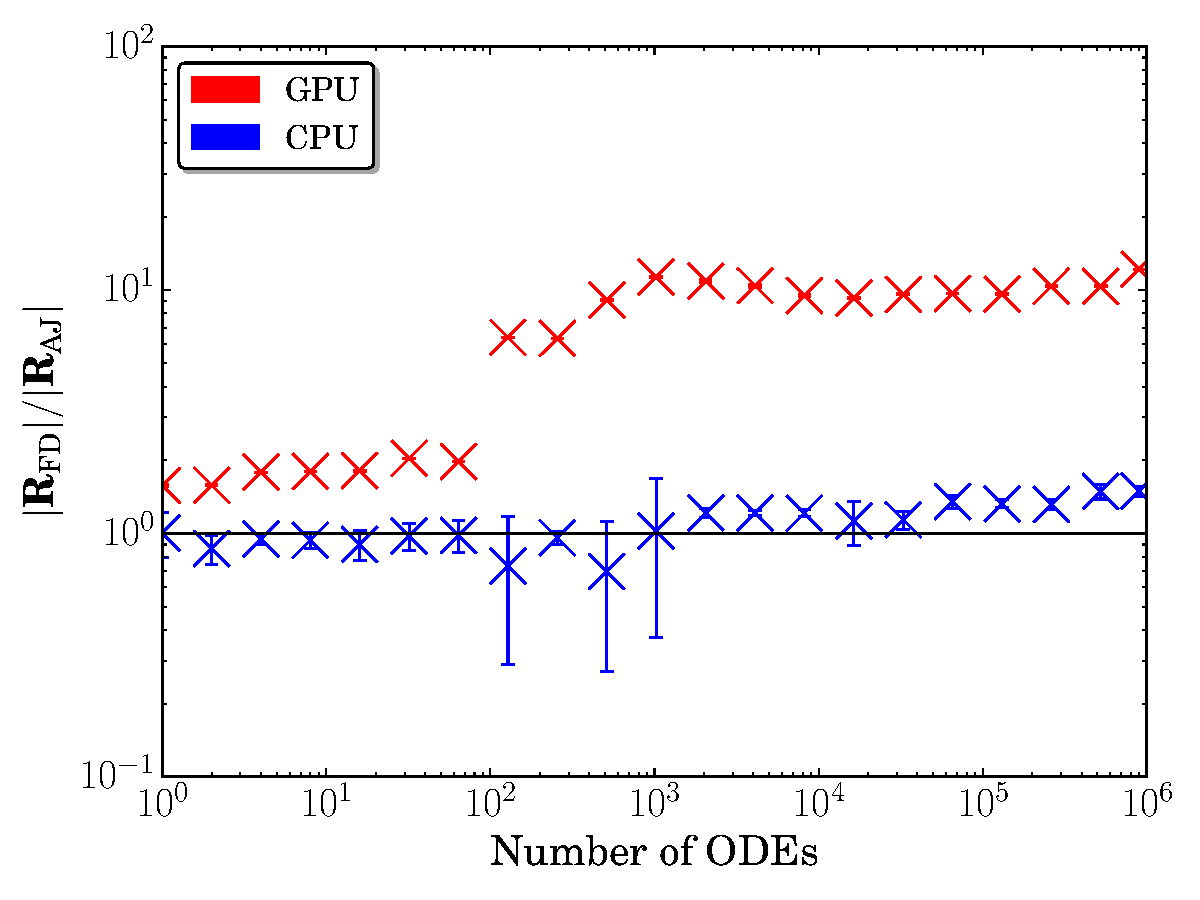
\includegraphics[width=\linewidth]{H2_1e-06_ajac_comp.pdf}
      \caption{\ce{H2}\slash\ce{CO} model with $\delta t = \SI{1e-6}{\second}$}   
      \label{F:AJ_h2_small}
  \end{subfigure}
  %\hfill
  \begin{subfigure}{0.49\textwidth}
      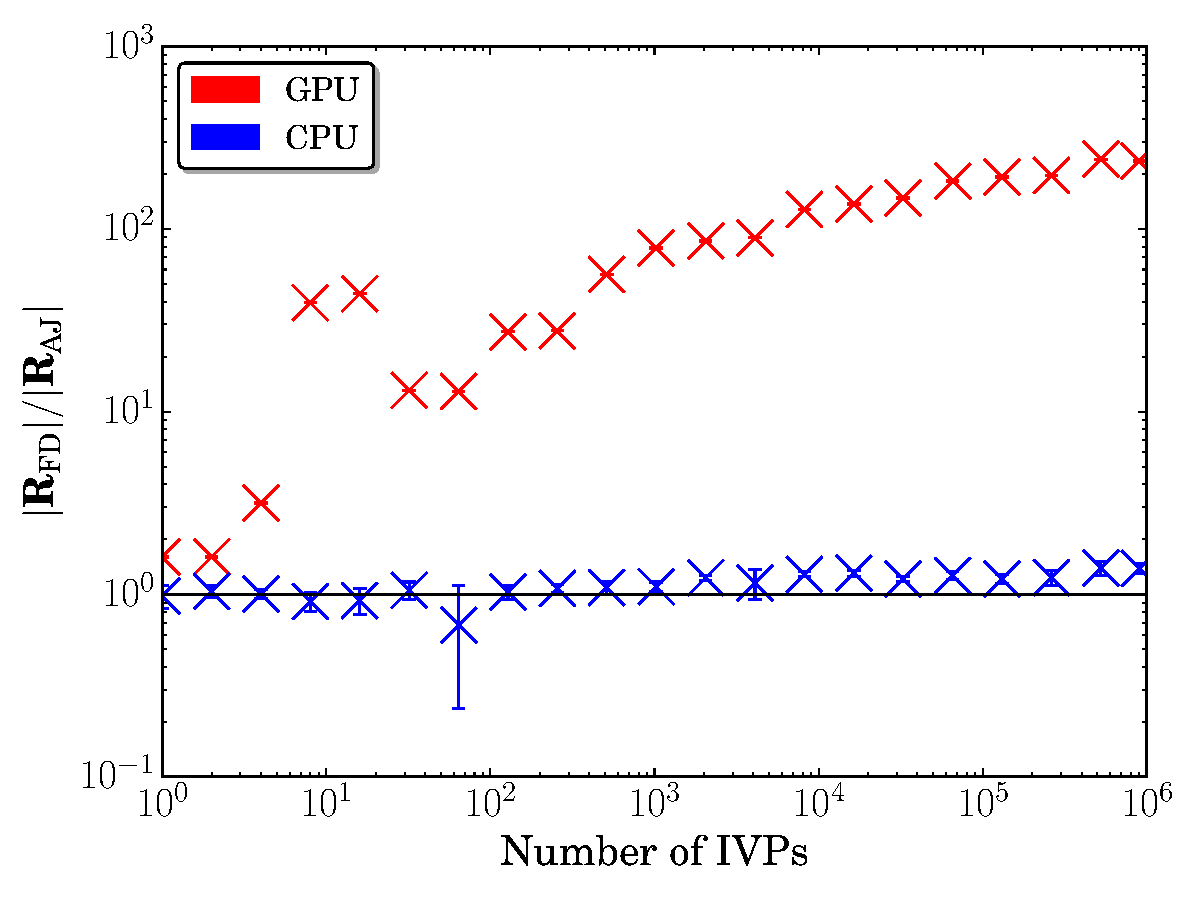
\includegraphics[width=\linewidth]{H2_1e-04_ajac_comp.pdf}
      \caption{\ce{H2}\slash\ce{CO} model with $\delta t = \SI{1e-4}{\second}$}
      \label{F:AJ_h2_large}
  \end{subfigure}
  \\
  \begin{subfigure}{0.49\textwidth}
      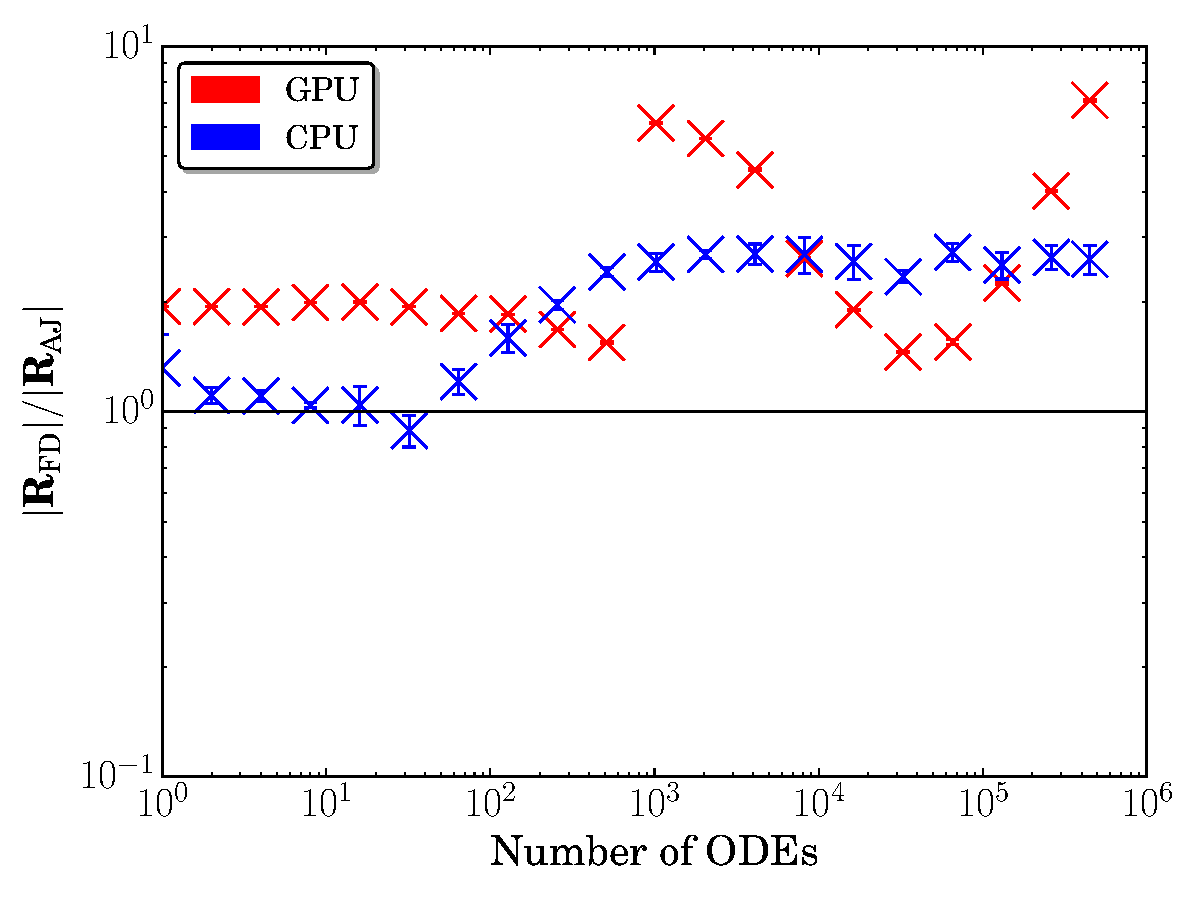
\includegraphics[width=\linewidth]{CH4_1e-06_ajac_comp.pdf}
      \caption{GRI-Mech 3.0 model with $\delta t = \SI{1e-6}{\second}$}
      \label{F:AJ_ch4_small}
  \end{subfigure}
  \caption{Ratio of the average finite-difference Jacobian based integrator runtime $\lvert\textbf{R}_{\text{FD}}\rvert$ to that of the analytical Jacobian runtime $\lvert\textbf{R}_{\text{AJ}}\rvert$ for the \texttt{Radau-IIA} (CPU\slash GPU) solvers.
  Error bars indicate standard deviation, and the horizontal lines show a ratio of one.}
  \label{F:AJ_comp}
\end{figure}

% \subsection{Effect of shared memory caching}
% \label{S:smem}
% 
% The effectiveness of the shared memory caching scheme was evaluated in several cases by comparing the mean runtime of the integrators using chemical source terms and analytical Jacobian subroutines generated with and without the caching algorithm enabled.
% We observed typical speedups of $\SI{5}{\percent}$ and $\SI{10}{\percent}$ for the smaller and larger global time-step sizes, respectively.
% This difference resulted from an increase in chemical source term and Jacobian evaluations required for the larger time-step size cases.
% Even larger speedup factors were observed in certain cases with the GRI-Mech 3.0 model: a \SI{24.4}{\percent} speedup with \texttt{exp4} for \num{131072} ODEs and the \SI{e-6}{\second} time-step size, and a \SI{13.2}{\percent} speedup with \text{Radau-IIA} for \SI{32768} ODEs and the \SI{e-4}{\second} time-step size.
% Thus, we recommend using this or a similar caching scheme in order to exploit shared memory in GPU integrators implemented on a per-thread basis.


%%%%%%%%%%%%%%%%%%%%%%%%%%%%%%%%%%%%%%%%%%%%
\section{Conclusions}
\label{S:conclusions}
%%%%%%%%%%%%%%%%%%%%%%%%%%%%%%%%%%%%%%%%%%%%

The large size and chemical stiffness of chemical kinetic models for fuels relevant to transportation and power generation applications traditionally requires the use of high-order implicit integrators for efficient solutions.
Past work showed orders-of-magnitude speedups for solution of nonstiff to moderately stiff chemical kinetic systems using explicit solvers on GPUs~\cite{Niemeyer:2011aa,Le2013596,Niemeyer:2014aa}.
In contrast, work on stiff chemical kinetic integration with implicit GPU solvers has been limited to specialized cases, or failed to surpass current CPU-based techniques~\cite{Stone:2013aa}.

This work demonstrated the performance of CPU- and GPU-based integration methods capable of handling greater stiffness, including an implicit fifth-order Runge--Kutta algorithm and two fourth-order exponential integration algorithms, using chemical source term and analytical Jacobian subroutines provided by the \texttt{pyJac} software~\cite{niemeyer_2016_51139,Niemeyer:2015ws,Niemeyer:2016aa}.
By comparing the performance of these algorithms using two chemical kinetics models, including hydrogen\slash carbon monoxide with 13 species and 54 elementary reactions~\cite{Burke:2011fh} and methane with 53 species and 325 reactions~\cite{smith_gri-mech_30}, and using two time-step sizes (\SI{e-6}{\second} and \SI{e-4}{\second}), we drew the following conclusions:
\begin{itemize}
 \item For time-step sizes relevant to large-eddy simulations, the GPU-based implicit Runge--Kutta method was roughly equivalent to the CPU-based implicit \texttt{CVODE} integrator running on \numrange{10}{35} CPU cores.
 \item At longer time-step sizes, the performance of all GPU-based integrators decreased significantly due to thread divergence.
 \item For the \ce{H2}\slash\ce{CO} model with a time-step size relevant to Reynolds-averaged Navier--Stokes simulations, the GPU-based Runga--Kutta solver performed nearly equivalent to \texttt{CVODE} running on \num{14} cores; for the GRI-Mech 3.0 model, the Runge--Kutta solver performance was only equal to \texttt{CVODE} on \num{2} cores.
 \item The exponential solvers were significantly less efficient than the implicit integrators on the CPU and GPU for all relevant cases.
 \item Using an analytical Jacobian matrix on the GPU is critical for efficient chemical kinetic integration due to thread divergence; speedups of \SIrange{8.09}{241.08}{$\times$} over a finite-difference-approximation were reached on the GPU, far surpassing the corresponding CPU speedup of \SIrange{1.58}{2.51}{$\times$}.
 \item Thread divergence and memory traffic were identified as key performance concerns for per-thread based GPU chemical kinetic integration algorithms.
\end{itemize}

Based on these results, we conclude that the exponential solvers poorly fit the SIMD acceleration paradigm due to high levels of thread divergence combined with the relatively high cost of integration steps due to Arnoldi iteration (as compared to other explicit integration techniques).
Instead, we recommend directing further focus on stiff explicit solvers such as (non-exponential) Rosenbrock solvers, explored for the CPU by Stone and Bisetti~\cite{stone2014comparison}, and inexact Jacobian W-methods~\cite{steihaug1979attempt,Schmitt2004}.
Further improvements to the analytical Jacobian code, e.g., by using a chemical kinetic system based on species concentrations to increase Jacobian sparsity, are likely to further increase performance of the developed algorithms.
However, this work clearly showed that thread divergence poses a large challenge to high performance of GPU-based integration techniques on a per-thread basis.
Our future work will therefore focus on a more comprehensive study of thread divergence, as well as developing methods to mitigate or eliminate its negative performance impact.
Finally, new integration techniques will be investigated and paired with work studying the selection of appropriate solvers based on estimated chemical stiffness.


%%%%%%%%%%%%%%%%%%%%%%%%%%%%%%%%%%%%%%%%%%%%%%%%%%%%%%%%%%%%%%%%%%%%%%
\section*{Acknowledgments}

This material is based upon work supported by the National Science Foundation under grants ACI-1534688 and ACI-1535065.

%% The Appendices part starts with the command \appendix;
%% appendix sections are then done as normal sections
\appendix
\setcounter{figure}{0}

% Fix for missing space between "Appendix" and letter
\renewcommand*{\thesection}{\appendixname~\Alph{section}}

\section{Supplementary material}
\label{S:supp}

The full \LaTeX\ source for this paper is available via a GitHub repository at \url{https://github.com/arghdos/GPU-Integration-Paper}, including the data and scripts needed to reproduce the figures here.

%%%%%%%%%%%%%%%%%%%%%%%%%%%%%%%%%%%%%
\section{Raw performance plots}
%%%%%%%%%%%%%%%%%%%%%%%%%%%%%%%%%%%%%
\label{S:raw}

In this section we present the plots of the raw, unnormalized performance data for completeness, as described in Section~\ref{S:results}.
Figures~\ref{F:raw_perf_H2CO} and \ref{F:raw_perf_CH4} show performance for the \ce{H2}\slash\ce{CO} and GRI-Mech 3.0 models, respectively.

\begin{figure}[htb]
  \centering
  \begin{subfigure}{0.49\textwidth}
      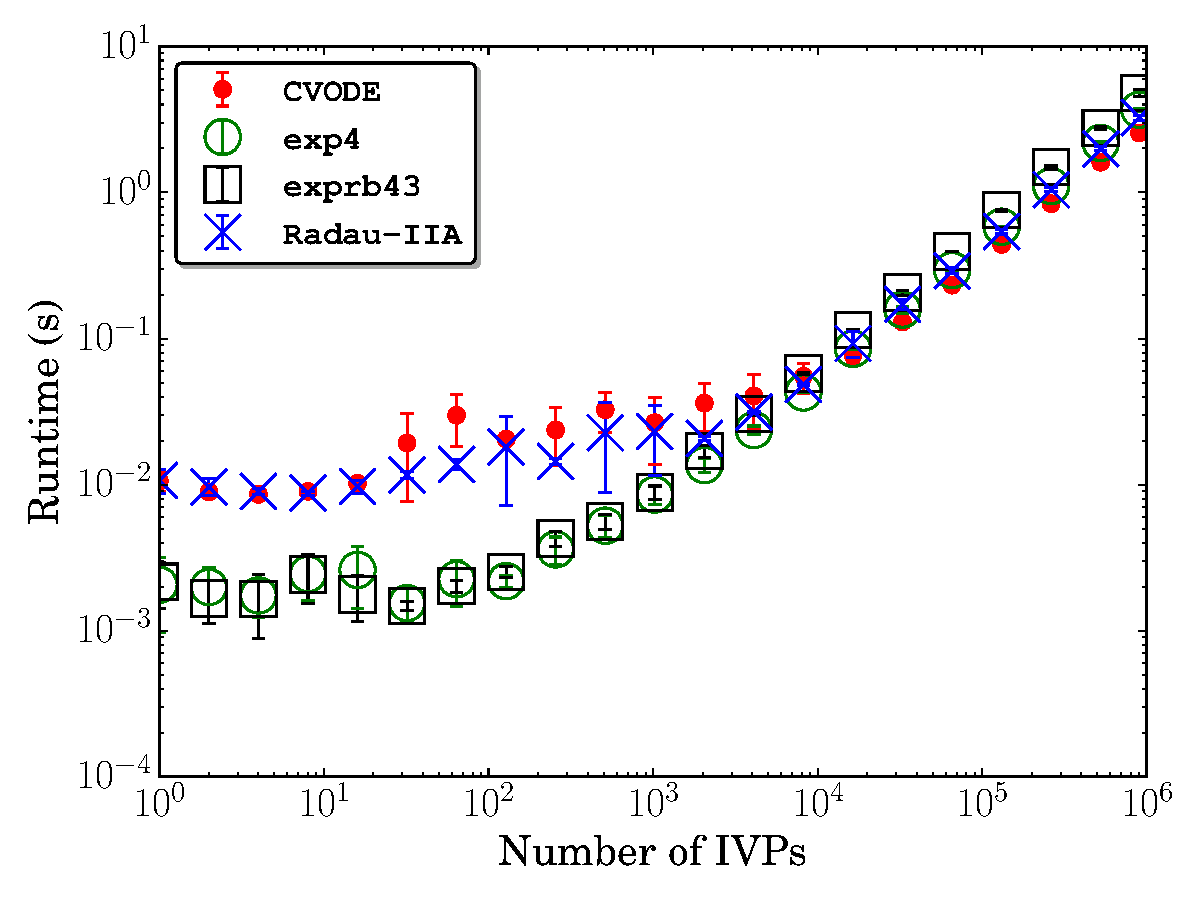
\includegraphics[width=\linewidth]{H2_1e-06_cpu_nonorm.pdf}
      \caption{CPU performance for $\delta t = \SI{e-6}{\second}$}
  \end{subfigure}
  %\hfill
  \begin{subfigure}{0.49\textwidth}
      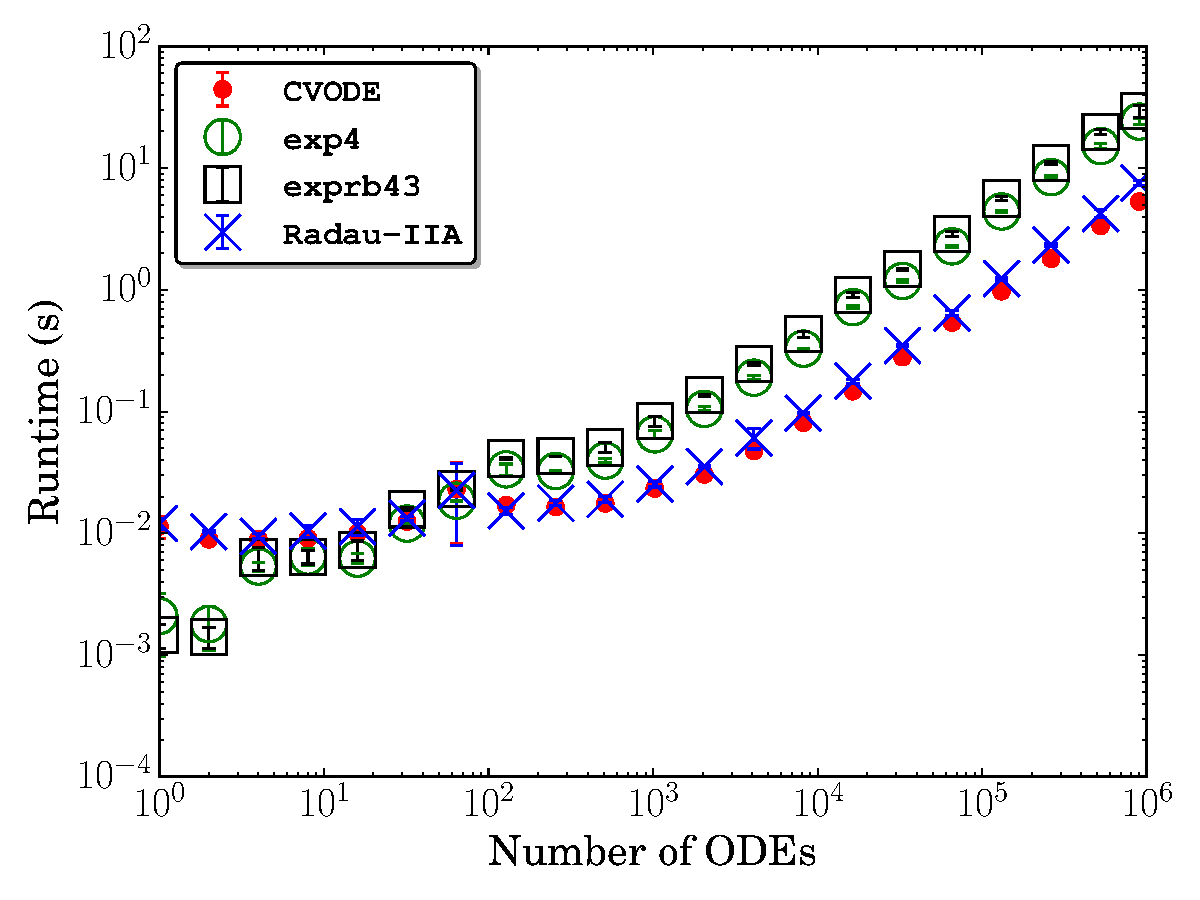
\includegraphics[width=\linewidth]{H2_1e-04_cpu_nonorm.pdf}
      \caption{CPU performance for $\delta t = \SI{e-4}{\second}$}
 
  \end{subfigure}\\
  \begin{subfigure}{0.49\textwidth}
      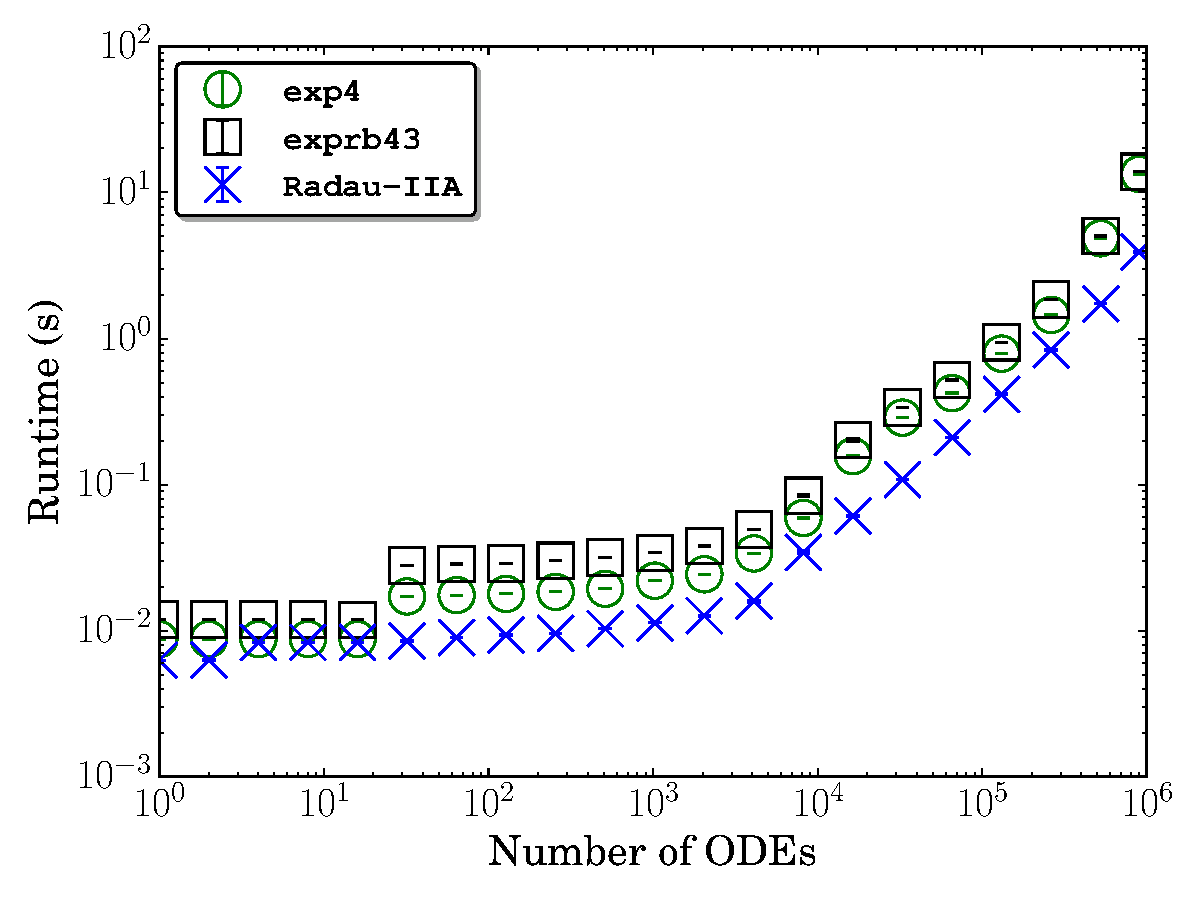
\includegraphics[width=\linewidth]{H2_1e-06_gpu_nonorm.pdf}
      \caption{GPU performance results for $\delta t = \SI{e-6}{\second}$}
  \end{subfigure}
  %\hfill
  \begin{subfigure}{0.49\textwidth}
      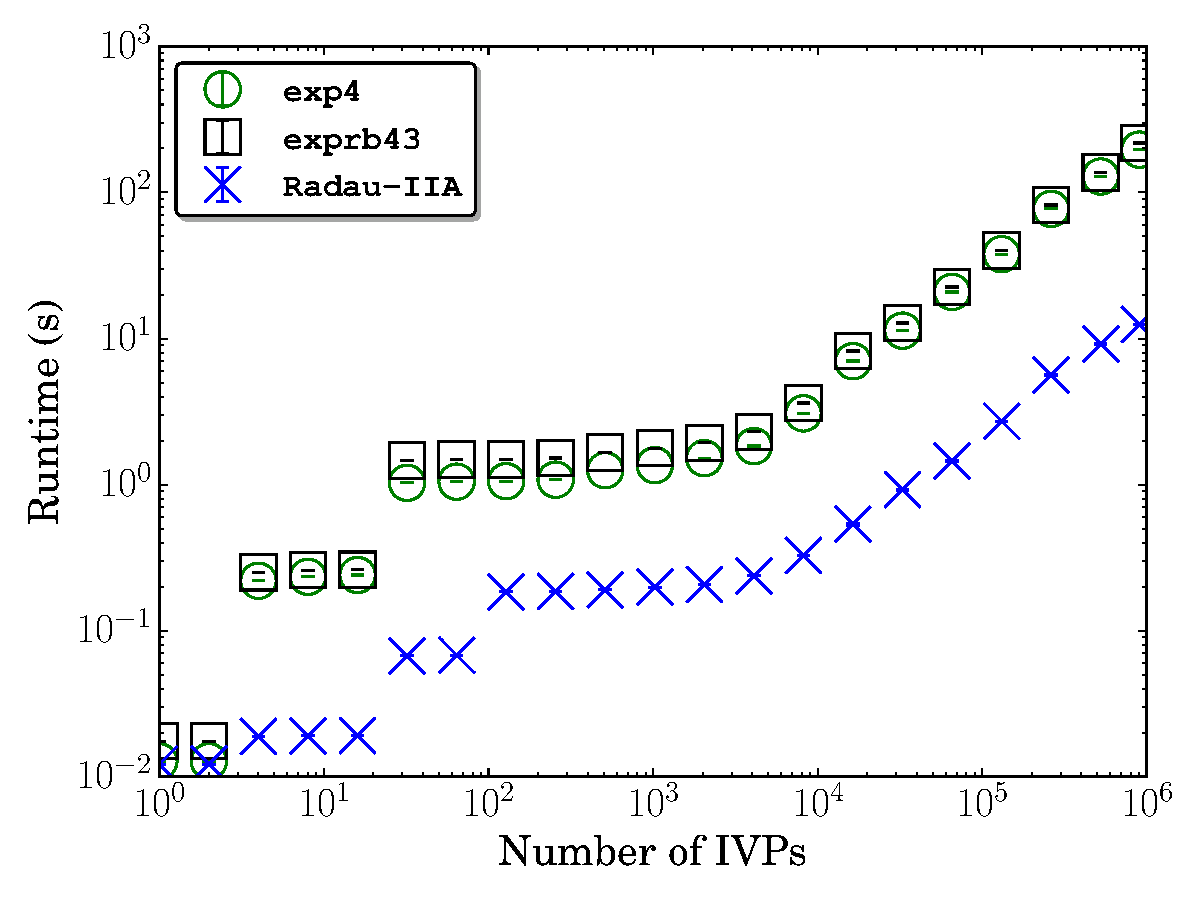
\includegraphics[width=\linewidth]{H2_1e-04_gpu_nonorm.pdf}
      \caption{GPU performance results for $\delta t = \SI{e-4}{\second}$}
  \end{subfigure}
  \caption{Average (unnormalized) runtimes of the integrators on the CPU and GPU for the \ce{H2}\slash\ce{CO} model at two different global time-step sizes.
  Error bars indicate standard deviation.}
  \label{F:raw_perf_H2CO}
\end{figure}

\begin{figure}[htb]
  \centering
  \begin{subfigure}{0.49\textwidth}
      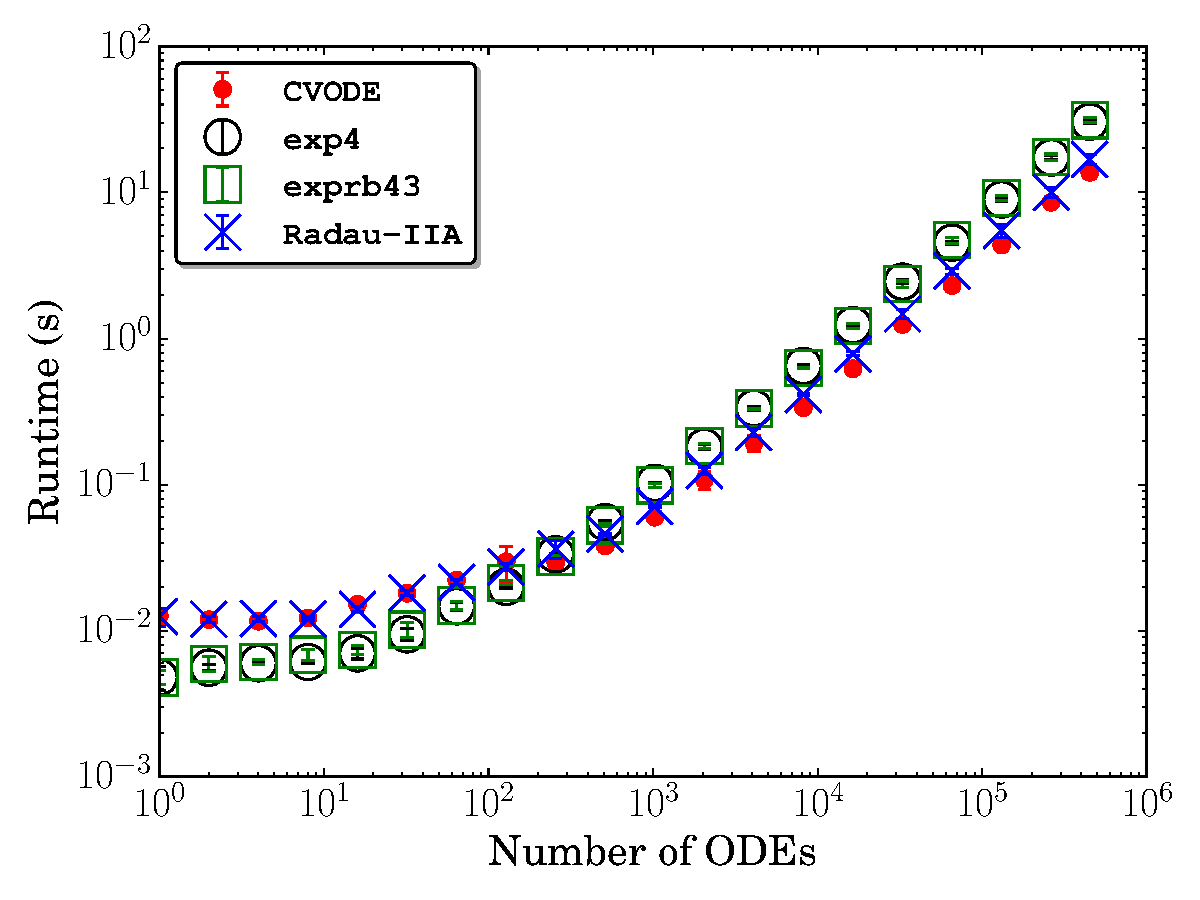
\includegraphics[width=\linewidth]{CH4_1e-06_cpu_nonorm.pdf}
      \caption{CPU performance for $\delta t = \SI{e-6}{\second}$}
  \end{subfigure}
  %\hfill
  \begin{subfigure}{0.49\textwidth}
      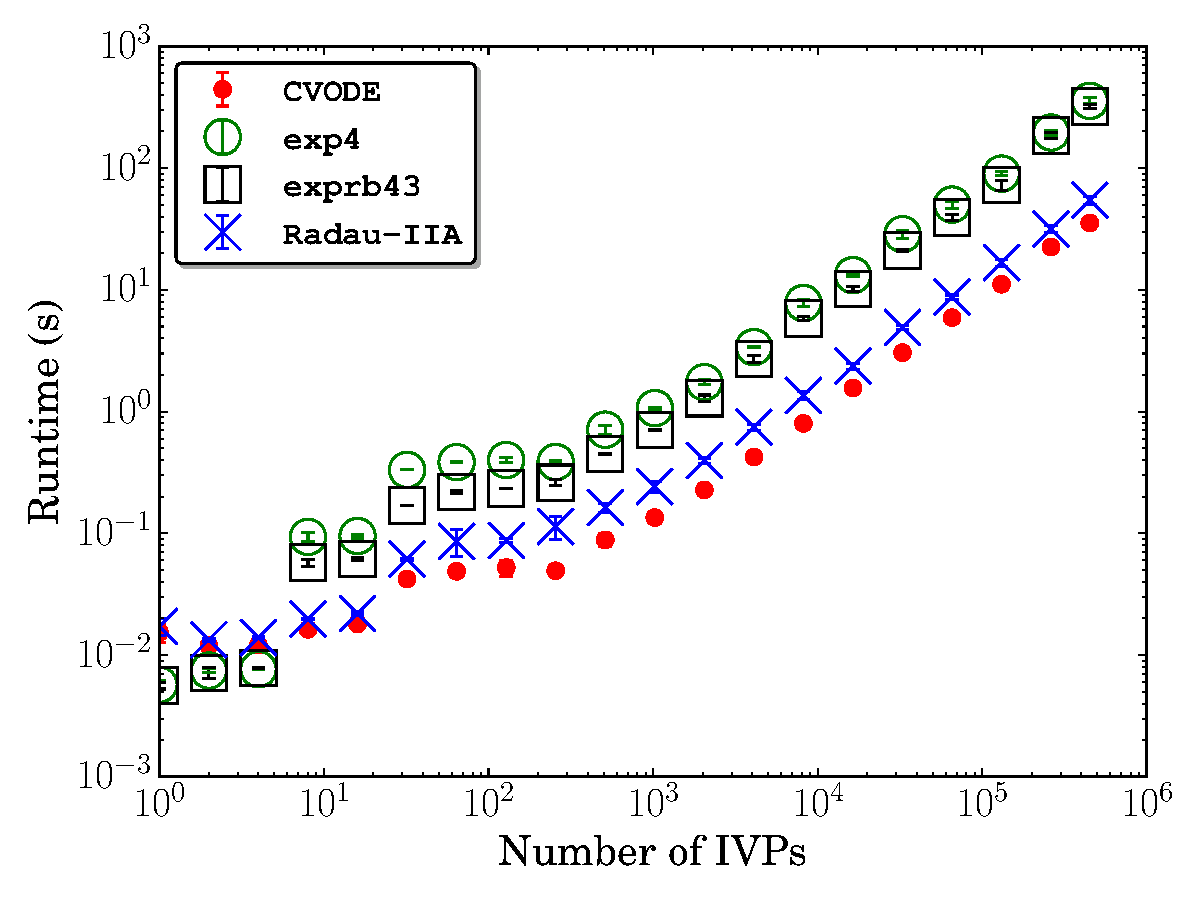
\includegraphics[width=\linewidth]{CH4_1e-04_cpu_nonorm.pdf}
      \caption{CPU performance for $\delta t = \SI{e-4}{\second}$}
  \end{subfigure}\\
  \begin{subfigure}{0.49\textwidth}
      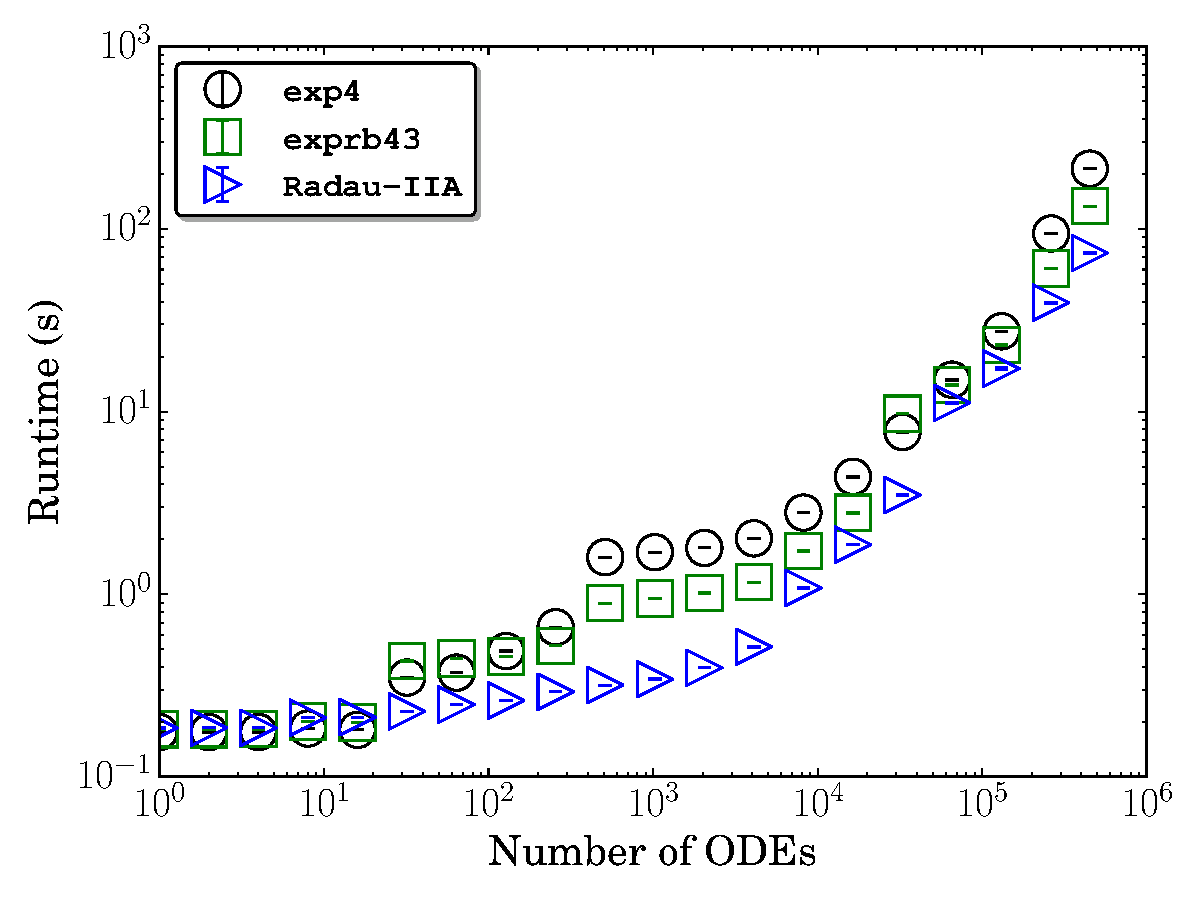
\includegraphics[width=\linewidth]{CH4_1e-06_gpu_nonorm.pdf}
      \caption{GPU performance results for $\delta t = \SI{e-6}{\second}$}
  \end{subfigure}
  %\hfill
  \begin{subfigure}{0.49\textwidth}
      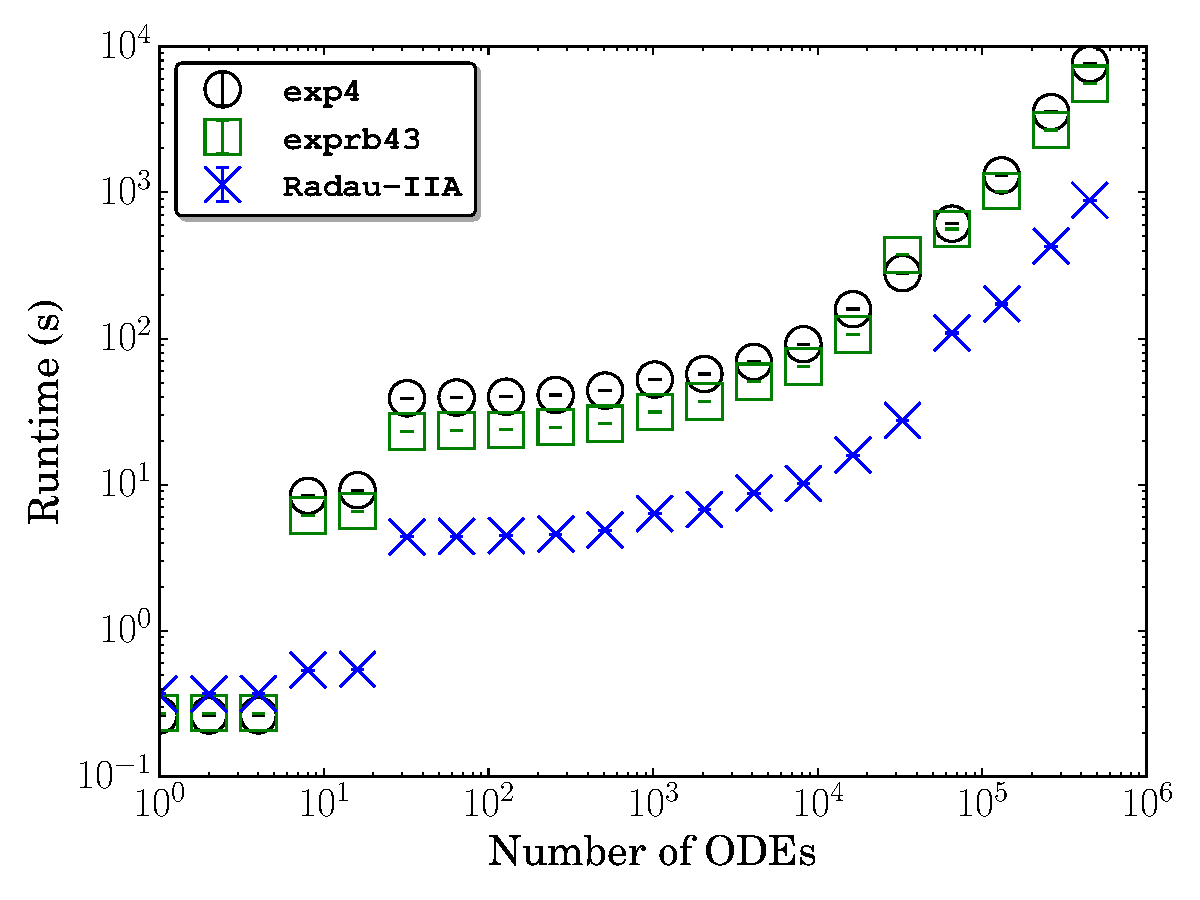
\includegraphics[width=\linewidth]{CH4_1e-04_gpu_nonorm.pdf}
      \caption{GPU performance results for $\delta t = \SI{e-4}{\second}$}
  \end{subfigure}
  \caption{Average (unnormalized) runtimes of the integrators on the CPU\slash GPU for the GRI-Mech 3.0 model at two different global time-step sizes.
  Error bars indicate standard deviation.}
  \label{F:raw_perf_CH4}
\end{figure}

\clearpage

\bibliography{GPU-integrator-paper}
\bibliographystyle{elsarticle-num}

\end{document}
